%% \documentclass[sigplan, 10pt]{acmart}
\documentclass[]{sig-alternate-10pt}

\usepackage{enumitem}
\setlist{leftmargin=5.5mm}
\usepackage{array}
\usepackage{booktabs} % For formal tables
\usepackage{xspace}
\usepackage{multirow}
\usepackage{makecell}
\usepackage{graphicx,amssymb,amsmath,endnotes}
\usepackage{ulem}
\usepackage{subcaption}
% \usepackage[tight]{subfigure}
\usepackage{fancyhdr}
\fancyhead{}
\fancyfoot{}
\fancyfoot[C]{\thepage}
\usepackage{textcomp, libertine}
\usepackage{hyperref}
\usepackage{soul,xcolor}
\usepackage{url}
\def\UrlBreaks{\do\/\do-}
\newcommand{\burl}[1]{\small{\url{#1}}}
\renewcommand{\UrlFont}{\ttfamily\small}
% Copyright
% \setcopyright{none}
% \renewcommand\footnotetextcopyrightpermission[1]{}	% Remove this in camera ready
% \settopmatter{printfolios=true} 
% \settopmatter{printacmref=false}
\pagestyle{plain}
\normalem
\fancyfoot{}
%\setcopyright{acmcopyright}
%\setcopyright{acmlicensed}
%\setcopyright{rightsretained}
%\setcopyright{usgov}
%\setcopyright{usgovmixed}
%\setcopyright{cagov}
%\setcopyright{cagovmixed}

% DOI

% ISBN

%Conference
% These commands are optional
%\acmBooktitle{Transactions of the ACM Woodstock conference}
\sloppy
\begin{document}
%\title{Morning Star: Accurate Power Modeling of OLED Displays on Modern Smartphones}
\title{
  {\it \LARGE How much battery does dark mode save?}\\
    An Accurate OLED Display Power Profiler
    for Modern Smartphones}

  % Accurate Power Modeling of OLED Displays


\author{
% \xspace
%% If anonymous submission change id in the acmart.cls line num 1117
Paper ID: 128, pages = 12+2
% Pranab Dash
% Y. Charlie Hu
} 


\newcommand{\oldstuff}[1]{}
\newcommand{\yes}{$\checkmark$}
\newcommand{\limited}{Limited}
\newcommand{\no}{$\times$}
% \definecolor{gray}{rgb}{0.5,0.5,0.5}
\newcommand{\etc}{\emph{etc.}\xspace}
\newcommand{\etcc}{\emph{etc.}}
\newcommand{\ie}{\emph{i.e.,}\xspace}
\newcommand{\eg}{\emph{e.g.,}\xspace}
\newcommand{\etal}{\emph{et al.}\xspace}
\newcommand{\SmallCrunch}{\vspace{-0cm}}
\newcommand{\smallcrunch}{\vspace{-0cm}}

\renewcommand{\paragraph}[1]{\smallskip\noindent{\bf{#1}}}

%\definecolor{purple}{RGB}{127,0,127}

\newcommand{\questionaj}[1]{{\color{red} \textbf{questionAJ: #1}}}
\newcommand{\updated}[1]{{\color{red} {}}}
%\newcommand{\updated}[1]{{\color{red} {updated: #1}}}
\newcommand{\editaj}[2]{{\sout{#1}\color{red} {#2}}}
\newcommand{\removeaj}[2]{{\color{red}{\textbf{Remove following:}}}{\sout{#1}}	{\color{red} {\textbf{Because} #2}}}
\newcommand{\addaj}[1]{{\color{red} {ADD?: #1}}}
%\newcommand{\highlight}[1]{{\color{blue}#1}}

\newcommand{\insitu}{{\em in situ}\xspace}

\newcommand{\name}{{\sc PFOP}\xspace}
\newcommand{\namee}{{\sc PFOP}}
\newcommand{\ychurm}[1]{{\hspace{-0.2cm}}}

\newcommand{\panic}[1]{\vspace{-#1 plus 1pt minus 1pt}}
\newcommand{\panictwo}[1]{\vspace{-#1 plus 2pt minus 2pt}}

% \newcommand{\appwithlink}[0]{\href{https://play.google.com/store/apps/details?id=com.pdeveloper.pcav5}{~\name~}}
\newcommand{\appwithlink}[0]{\name~\cite{PFOP}~}

% \newcommand{\nsection}[1]{\panictwo{0pt}\section{#1}\panictwo{0pt}}
% \newcommand{\nsubsection}[1]{\panictwo{0pt}\subsection{#1}\panictwo{0pt}}
% \newcommand{\nsubsubsection}[1]{\panictwo{0pt}\subsubsection{#1}\panictwo{0pt}}

\newcommand{\flow}{flow\xspace}
\newcommand{\comment}[1]{{\it #1}}
\newcommand{\forjnl}[1]{{}}
\newcommand{\dcomment}[1]{{\it \color{red} #1}}
\newcommand{\dacomment}[1]{{\it \color{blue} #1}}
\newcommand{\dtext}[1]{{\it #1}}

\newcommand{\expr}[1]{{\color{red} Experiments: #1}}


\newcommand{\coflowone}{C_1}
\newcommand{\coflowtwo}{C_2}
\newcommand{\nexuserror}{19.4\%\xspace}
\newcommand{\pixelerror}{23.8\%\xspace}
\newcommand{\motoerror}{13.4\%\xspace}

\newcommand{\pixeltwoerrorreduction}{4.9$\times$\xspace}
\newcommand{\motozthreeerrorreduction}{4.2$\times$\xspace}
\newcommand{\pixelfourerrorreduction}{3.7$\times$\xspace}


\newcommand{\revv}[1]{{#1}}
\newcommand{\tabincell}[2]{\begin{tabular}{@{}#1@{}}#2\end{tabular}}
\newcolumntype{M}[1]{>{\centering\arraybackslash}m{#1}}

\setstcolor{red}
\maketitle
\begin{abstract}

By omitting external lighting, OLED display significantly reduces the
power draw compared to its predecessor LCD and has gained wide
adoption in modern smartphones.  The real potential of OLED in saving
phone battery drain lies in exploiting app UI color design, \ie how to
design app UI to use pixel colors that result in low OLED display
power draw.
%   Doing so, however, requires a per-frame OLED power
%   profiler than can accurately estimate the OLED power draw of each
%   displayed frame on a given device and its breakdown among the various
%   constituting UI components.
In this paper, we design and implement
an accurate per-frame OLED display power profiler, \namee, that helps
developers to gain insight into the impact of different app UI design
on its OLED power draw, and an enhanced Android Battery that
helps phone users to understand and manage phone
display energy drain, for example, from different app and display
configurations such as dark mode and screen brightness. A major challenge in
designing both tools is to develop an accurate and robust OLED display
power model.  We experimentally show that the linear-regression-based
OLED power models developed in the past decade cannot capture the
unique behavior of OLED display hardware in modern smartphones which have
a large color space and propose a new piecewise power model that 
achieves much better modeling accuracy than the prior-art
by applying linear regression in each small regions of the vast color
space.
Using the two tools, we performed to our knowledge the first power
saving measurement of the emerging dark mode for a set of 6 Google
Android apps.

%  We demonstrate how the \name profiler can be used by app developers to
%  easily quantify the impact of dark mode on the OLED
%  power draw  and further gain insight into the OED power breakdowns
%  at the UI-component granularity.

\if 0
Accurate OLED power modeling is essential in power management such
as energy profiling and optimization of mobile apps and devices.
Since OLED power draw depends on the colors of the pixels displayed,
accurate modeling of OLED displays is challenging as modern phone OLED
displays come with millions of pixels, each with a huge color space
($256^3$).  In this paper, we first present a measurement study to
characterize the power behavior of OLED displays on modern
smartphones, which illustrates the limitations of the prior OLED power
models. We then present a novel OLED power model that overcomes the
challenges presented by the unique OLED display power behavior on
modern phones. We show the new model reduces the OLED power prediction error
of the prior art from
\nexuserror, \pixelerror, and \motoerror,
% 5.8\%, 23.8\%, and 13.4\%
to 3.3\%, 3.3\%, and 2.9\% across 3 recent generations of Android phones.
Third, we develop a per-frame OLED power profiler that accurately breaks down the
OLED power in displaying a frame among the UI components.
Finally, using the OLED power profiler, we quantify
the OLED and whole phone power savings for a set of 9 Google and Android system apps that
recently rolled out with support for cm``dark mode'' -- the latest power saving
scheme embraced by
% dominating mobile OS players such as
both Android and
iOS.  Our study shows that at brightness level 50\%
switching to dark mode reduces the OLED
power draw on average by 45\%, 22\% and 21\% on Nexus 6,
Pixel 2 and Moto Z3 for the set of
Google apps which translates into 13\%, 6\% and 7\%
average total phone power draw reduction on the 3 phones, respectively.
The power savings are significantly higher at 100\% brightness level.
\fi

\end{abstract}

\pagestyle{plain}
\thispagestyle{empty}

\vspace{-0.01in}

\section{Introduction}
\label{sec:intro}

Optimizing the battery drain of mobile apps helps to extend the
mobile device battery life which is critical to the mobile experience
of the 5+ billion phone users (over half are smartphones)~\cite{gsma2019}.
Optimizing the battery drain of mobile
apps requires optimizing the battery drain of all power-hungry
device components, including CPU, GPU, display, WiFi/LTE,
GPS, and hardware decoder. After over a decade of phone evolution, display
has remained as one of the major power-draining components in modern
smartphones~\cite{dong2009current,dong:2011chameleon,chen:2013:display,wan:2017:displayenergy,chen:2016:dac,chan:2016:image,crayon:eurosys16}.

% The display technology has also evolved over the years.
The latest display technology, Organic light-emitting diode (OLED)~\cite{oled:2003,oled:2004},
uses light-emitting diode as pixels and therefore omits the need for
external backlight used in its predecessor LCD, and in doing so
provides much better power efficiency than LCD.  Due to its power
efficiency and several other advantages (thinner, lighter, and more
flexible) over LCD and LED, OLED has seen wide adoption in high-end and mid-range
smartphones.

Since the OLED power draw is directly related to the displayed
content, the real potential of OLED in terms of power savings lies in
exploiting the app UI color design, \ie how to design the app UI 
to use pixel colors that result in less OLED display power draw.
These include manual designs by app developers as well as
automatic color transformations~\cite{dong:ispled09,dong:2011chameleon,crayon:eurosys16}.
One of the extreme examples of color transformation to save display energy of mobile
devices is the recent wide adoption of 
dark-themed color contents, known as dark mode,\footnote{An old idea first supported in modern OS as early as 1991 (Apple's System 7 OS).}
% which are known to draw much less power than white-theme color contents. 
%  the mobile industry did not catch on until late 2018
by both Android and iOS which added dark mode as one of major
features in their 2019 OS
update~\cite{googledevsummit2018,appleaccouncedarkmode}, and app
vendors who quickly rolled out dark mode UI options in their latest
app releases~\cite{darkModeActicle1,darkModeActicle2,darkModeActicle3,darkModeActicle4,darkModeActicle5,darkModeActicle6,darkModeActicle7}.

Despite the industry's major push for dark mode, it remains unclear
how much power and energy savings dark mode will bring to the apps, as
the OLED display power saving from switching from the normal (or
light) to dark mode depends on the displayed content, which can vary
significantly from one app to another, and from one app activity to
the next. More generally, the industry is lacking an OLED display
power profiling tool that can accurately estimate the OLED display
power draw and attribute it to the individual UI components.  Such a
tool will enable an app developer to gain instant insight into how different
UI designs affect the OLED display power draw in running the app on
specific mobile devices and optimize the app UI design accordingly.

\if 0
In this paper, we undertake to our knowledge the first measurement
study of the energy savings of dark mode for a set of preinstalled Google/Android system
apps that recently rolled out support for dark mode.
% ,as well as the upcoming Android Q (using its beta release) dark theme.
\fi

In this paper, we present the design and implementation
of two OLED power management tools:
an accurate per-frame OLED display power profiler, \namee, that helps
developers to gain insight into the impact of different app UI designs
on its OLED power draw, and an enhanced Android Battery called Android Battery+ 
(or Battery+ for short) that
helps phone users to understand and manage phone
display energy drain, for example, from different app and display
configurations such as dark mode and screen brightness. A major challenge in
designing both tools lies
in designing an accurate and robust
OLED power model that accurately estimates the display power draw
as a function of the displayed content on any device.
%   , as either the
%   external power meter or the internal power sensor can only measure the
%   total phone power draw by all its active components; (2) We need to
%   identify all the UI components of a displayed frame, \eg separating
%   dynamic objects from static objects, in order to calculate 
%   the OLED power draw by each UI component.

\if 0
An accurate OLED power model enables app developers to
% isolate and
quantify the OLED display power/energy savings which has many
applications, such as studying the power savings from switching to
dark mode for any apps running in the lab or ``in the wild'' on real
users' phones
% \footnote{We have developed an app that records the
% screen and accurately caculates the OLED energy drain throughout the   day.}
and more generally energy profiling of mobile
apps~\cite{appscope,zhang2010accurate,shye2009into,pathak:eurosys12,mittal:mobicom12,androidprofiler}
which performs component-wise energy accounting at the app source-code
level.
\fi


Since power modeling of OLED display has been studied
over the past decade, first on external display then
earlier smartphones~\cite{dong2009current,kim2013runtime,park2015accurate},
we first study {\em if the prior-art power models of OLED display proposed
  in the past decade can accurately capture the power behavior of OLED
  displays on modern smartphones.}  To answer this question, we
conduct a measurement study to characterize the power behavior of OLED
displays on three representative smartphones from 
three recent generations, Pixel 2 (2017), Moto Z3 (2018), and Pixel 4 (2019).
%
Our measurement study reveals
unique power draw behavior of modern phone OLED displays: (1) The OLED
display power draw violates the superposition property observed
in~\cite{dong2009current}, \eg the power draw in displaying
the white color can be far less than the simple summation of those in
displaying the three base colors: red, green and blue (after removing
base power).  (2) The OLED
display power often violates the  monotonicity principle, that
the power draw in displaying canonically larger RGB values in the color
space should be higher.
\forjnl{(3) New features in
recent phones such as color mode, color correction
as well as adjusting the hardware brightness button
directly affect the OLED display power draw
via color transformation in hardware composer,
which does not change the pixel
values in the frame buffer (what is recordable from the OS-provided
API).
}
The two findings suggest that previously proposed
linear and non-linear OLED power models are unlikely to achieve high
prediction accuracy, as confirmed by our experiments.
\forjnl{
  and the third suggests that any OLED power model based on frame buffer pixel values
needs to adjust for color transformations that can happen in the hardware composer.
}

Second, we study {\em how to develop new practical OLED power models that
  can accurately and robustly capture the power behavior of modern smartphone OLED
  displays.}  To develop such a power model,
we first unearth the root cause for why previous models fail:
%we    plot the OLED
%    power draw in displaying static chromatic images of pixels that span
%    the 3-D color space and found
% we first uncovered that the fundamental reason that
linear regression of subpixel power functions (which are linear in linear RGB
values)
% \footnote{Linear RGB values are RGB valeus with gamma-correction.}, respectively)
cannot capture the OLED power behavior of modern OLED displays
% is that
because any linear combinations of linear functions 
can only fit a flat plane, while the OLED power
values across the color space do not fall into a flat plane.

Our new OLED power model is based on a key observation that though the
pixel power values in the color space do not fall in a plane,
they form a reasonably smooth surface.  Therefore, if we cut
the 3-D color space into small subgrids, the pixel power values within
each subgrid are likely to fit closely in a flat plane and thus can be
fitted well using linear regressions of the (linear) subpixel power
functions. We experimentally show that our new piecewise OLED power model reduces the
OLED prediction error of the prior art~\cite{park2015accurate} by
5.1$\times$, 5.5$\times$ and 4.4$\times$ for dark
and 4.2$\times$, 2.3$\times$ and 2.5$\times$ for light mode for the three phones,
respectively, for a set of activities across 6 popular google apps.
%% NLM model vs P-NLM model

% 7.2$\times$-4.6$\times$,
% from
% \nexuserror, \pixelerror, and \motoerror,
% down to 3.3\%, 3.3\%, and 2.9\% on the three phones,
% respectively, for a set of 100 images with diverse graphical content.

%   The new OLED power model has many potential applications, such as
%   building fine-grained energy which requires accurate power model for
%   every power-hungry phone component.
%   profiler~\cite{appscope,zhang2010accurate,shye2009into,pathak:eurosys12,mittal:mobicom12,androidprofiler}.

Third, we design and implement the two tools on top of our new OLED
power model. \name accurately breaks down the OLED display power in
displaying a frame among its UI components and faces the challenge of
identifying all the UI components of a displayed frame, \eg an app
activity.
% , in order to calculate the OLED power draw by each UI component.
We design \name to use only standard Android services so
it is portable to any unmodified Android versions.
% {without superuser access}.  
Battery+ replaces
the simple screen energy accounting of Android Battery with an
accurate, per-app screen power and energy estimator.  Like Android
Battery, it runs in real time in the background and thus needs to have low
overhead. We carefully apply pixel sampling to both screen recording
and model application to control its average CPU utilization to be
only 1.1\%, 0.9\%, and 0.6\% on Pixel 2, Moto Z3, and Pixel 4, respectively,
while minimally affecting the power estimation accuracy.

%  to identify UI components
%  , that accurately breaks down the OLED power draw
% in displaying a frame among its constituting UI components.  We design
% \name to be easy-to-use -- it runs as an app,
% portable to different Android versions -- it only uses standard Android services
%  to identify UI components, and efficient by using pixel sampling -- analyzing a frame takes
% less than 8 seconds on all three phones.

%    , and an Enhanced
%    Android Battery that accurately measures the screen energy of all apps
%    running on the phone and assists phone users to adjust screen
%    brightness to elongate battery life.

Finally, 
%   how the OLED power profiler can be used by
%   developers and phone users to understand and optimize the battery drain
%   of different app UI designs,
we showcase the usage of the two tools by performing a case study of the dark mode
power saving that answers {\em how much does dark mode reduce the
  OLED display power draw and energy drain for real apps?}  In
particular, we study the power consumption of a set of 6
 Google apps {(each with 1B+ downloads)} in two ways.  First, {\em from the phone user's
  perspective,} we analyze the power draw of each Google app under a
typical user interaction using Battery+.
%   that lasts about 40 seconds which is driven
%   by UIAutomator 2~\cite{uianimator} and Appium~\cite{appium} to ensure
%   the same user interactions are carried out under light and dark modes.
Battery+ shows that (1) switching from light to dark mode
significantly reduces the average OLED power draw across all apps,
though the reduction varies significantly among the apps and the phones, ranging
between 4\%-34\% (average 24\%), 12\%-35\% (average 25\%), and
12\%-24\% (average 19\%) at the 50\% brightness level,
%    , and
%    48\%-67\% (average 58\%), 
%    64\%-81\% (average 72\%),
%    and 62\%-76\% (average 68\%) for 100\% brightness level,
on the 3 phones, respectively.  (2) The significant OLED power reduction
translates into moerate reduction in the total phone power draw, ranging between
-3\%-15\% (average 7\%),
-12\%-13\% (average 5\%),
and 0\%-15\% (average 10\%) at the 50\% brightness level
%  2\%-29\% (average 15\%),
%  16\%-46\% (average 32\%),
%  and 24\%-59\% (average 43\%)
across the apps on the 3 phones, respectively.

Second, {\em from the app developer's perspective}, we use \name to analyze how
much power the UI design change of each activity in dark mode saves in
the 6 Google apps.
%  We manually navigate each of
%  the apps to stop at all its major activities when running under 
%  dark and light mode, and capture the screen via screencap, and
%  then apply our new OLED power model to the captured screens to
%  calculate the OLED power draw.
\if 0
(1) Switching from light mode to dark mode significantly reduces the OLED power
draw of the app activities, ranging between 48\%--67\% (average 58\%),
64\%--81\% (average 72\%), and 62\%--76\% (average 68\%),
for brightness level 100\% across the apps on the 3 phones, respectively,
%  (2) The drastic OLED power saving in switching to dark mode 
which translates into significant saving of whole phone power draw,
on average 26\%, 39\%, and 47\% across the apps on the 3 phones, respectively.
(2) More importantly,
\fi
Our study shows how
\name quantifies and displays the power saving for each UI component
in switching to the new color scheme in dark mode, allowing app developers
to easily experiment with the design-power tradeoff of
alternative dark mode designs.

%  To our best knowledge, this is the first public measurement study of
%  OLED display power savings by dark mode on smartphones.

% Fourth, {\em can we develop design guidelines for app vendors who are thinking about developing dark mode and want to estimate the potential energy saving before investing the development effort?} 

We summarize the contributions of our study as follows:
\begin{itemize}[leftmargin=*]
  \item We experimentally characterize the unique power draw behavior
    of OLED displays on 3 representative modern smartphones and show
    how they violate the underlying assumptions made in prior OLED
    power models proposed in the past decade.
  \item We propose a new piecewise OLED power model and experimentally
    show that it reduces the prediction error of the prior art by 
%    \pixeltwoerrorreduction,
%    \motozthreeerrorreduction, and
%    \pixelfourerrorreduction
5.1$\times$, 5.5$\times$ and 4.4$\times$ for dark mode
and 4.2$\times$, 2.3$\times$ and 2.5$\times$ for light mode 
    on Pixel 2, Moto Z3, and Pixel 4, respectively.
  \item Using our new model, we develop a per-frame OLED
    power profiler that enables developers to instantly understand the
    OLED power draw breakdowns of activity UI designs to guide UI power optimization and an enhanced Android Battery that enables phone users to
understand and manage phone
display energy drain, for example, from different app and display
configurations such as dark mode and screen brightness.
%     , and an
%     Enhanced Android Battery that accurately measures the screen
%     energy of all apps running on the phone and assists phone users to
%     adjust screen brightness to elongate battery life.  
  \item Using the two tools, we present to our knowledge
    the first public study of the OLED power and phone power
    savings in switching from light mode to dark mode for a
    set of preinstalled Google apps {(each with 1B+ downloads).}
  \end{itemize}




\if 0
Light-on-dark color scheme, or dark mode in short, refers to the color
scheme that uses light-colored text, icons, and graphical user
interface elements on a dark background.  While dark mode
is known to reduce the power on display technologies in general,
its saving on OLED is particularly pronounced, due to the unique power
characteristics of OLED displays.  For this reason, both Google and
Apple announced in late 2018 that dark mode would be made available on
Android and iOS devices. Since then an increasingly number of apps
(by toggling ``Enable Dark Theme'' in the app's settings) has rolled out
the dark mode option, and the Android system UI also added the dark
theme.

While it is generally understood that using dark color will lower the OLED
display power consumption, it is much less clear on how much
energy savings will dark mode bring to individual apps, as the
OLED display power saving in switching from light to 
dark mode depends on the displayed content and which may vary
significantly from one app to another. In this section, we conduct a
measurement study of the energy savings of dark mode for a set of
preinstalled Google apps which are hugely popular and thus will affect
a large number of mobile users by adopting dark mode.
The improved accuracy of the new model comes with negligible overhead:
64KB for storing 4K 4-coefficient linear regression models
and 678ms - 1100ms in applying the model to one complete frame on the 3 phones.

\fi

\section{Background}
\label{sec:back}

\if 0
The display technology used by mobile devices started from monochrome display
to liquid crystal display (LCD) to the present technology of organic
light-emitting diode (OLED).
In the LCD the brightness of the screen is regulated by a backlight. With the
advent by OLED the brightness was depended on the pixel with are lighted.
\fi

\paragraph{Frame rendering.}
% Figure~\ref{fig:arch} illustrates the frame rendering process in a
% typical modern smartphone.  After the GPU renders a new frame, \eg
% every 16.7ms at 60 FPS, the bitmap of the frame content is stored in
% the frame buffer and sent to the hardware composer. The hardware
% composer before sending the final bitmap to
% the hardware display.  Each unit of the bitmap describes the color of
% a pixel in the standard RGB (sRGB) color space, ($R, G,
% B)$, which specifies the intensities of the red, green, and blue base
% colors.  Modern displays come with 24-bit (8, 8, 8) RGB color setting,
% \ie each intensity ranges between 0 and 255.
Figure~\ref{fig:arch} illustrates the frame rendering process in a
typical modern smartphone~\cite{arch_graphicspipeline}.
After the GPU renders all the layers for the next frame
(for status bar, navigation bar, and app UI),
\eg every 16.7ms at 60 FPS, 
the bitmap of the frame content is stored in separate buffer queues.
%
Each unit of the bitmap describes the color of
a pixel in the standard RGB (sRGB) color space, ($R, G,
B)$, which specifies the intensities of the red, green, and blue base
colors.  Modern displays come with 24-bit (8, 8, 8) RGB color setting,
\ie each intensity ranges between 0 and 255.
%
SurfaceFlinger provides HardwareComposer HAL with a list of layers and
instructs it to compose the final frame sent to the display.
HardwareComposer HAL may perform additional color transformation to
generate the final frame.

If the Android screenrecord command is issued, SurfaceFlinger composes
the multiple layers from buffer queues into a frame
buffer~\cite{arch_surfaceflinger} sent to an additional virtual
display for screen recording. Note that such recorded frame buffers would not
include color transformation happening in HardwareComposer below.

%  The Hardware Composer HAL (HWC) composite buffers in the most
%  efficiently specific to device display hardware.


%  and may not be the true representation
%  of the device display, as it is handled by SufaceFlinger.  Hence, the
%  color mode, color correction and brightness changes are not captured
%  by virtual display.

\begin{figure}[tp]
  \centering
        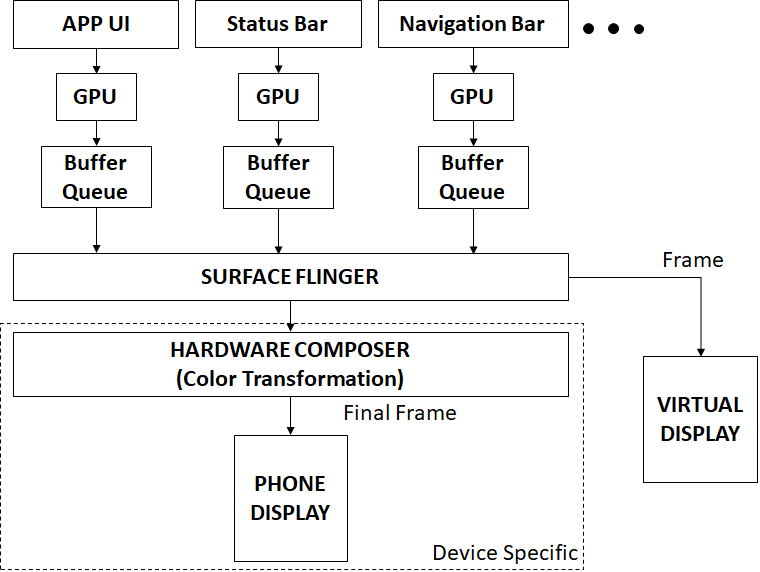
\includegraphics[width=0.45\textwidth]{./figure/1400_architecture.png}
        \vspace{-0.1in}
	\caption{Frame rendering in modern smartphones.}
        \vspace{-0.2in}
        \label{fig:arch}
\end{figure}

\forjnl{Organic light-emitting diode (OLED), also known as an organic EL
  (organic electroluminescent) diode~\cite{oled:2003,oled:2004}, is a light-emitting
diode (LED) in which the emissive electroluminescent layer is a film
of organic compound that emits light in response to an electric
current.}
%
\if 0
offer several
significant advantages: (1) OLED enables a greater contrast ratio and
wider viewing angle compared to LCD, because OLED pixels emit light
directly. In particular, OLED provides a deeper black level, since a
black OLED display emits no light, while
 LCD cannot show true black, since it filters the light emitted from a backlight.
 (2) OLED
 \fi
% Further, OLED pixel colors appear correct and unshifted, even as the viewing angle approaches 90° from the normal.
\forjnl{ The ability of OLED pixels to emit light omits the need for external
 backlight needed in LCD and provides much better power efficiency than LCD.
}


\paragraph{OLED display.}
Each pixel of an OLED display consists of three subpixels,
corresponding to red, green, and blue colors, which
can differ significantly in their luminance
efficacies~\cite{oled:2003,oled:2004}.  This is the reason why the color of a pixel determines
its power consumption and thus different display content (\eg different
app UI design) can result in very different OLED display power draw.
\forjnl{This is in stark contrast with LCD displays where the (external) back
lighting dominates the whole display power.
}

In addition to the panel of addressable pixels, the total OLED display
power consumption is additionally affected by the control circuitry
that generates the control and data signals for the panel based on
display contents. Different circuitry implementation can potentially
result in different power draw.
%   There are two main families of OLED, based on small molecules
%   and polymers, respectively.
%   Adding mobile ions to an OLED creates a
%   light-emitting electrochemical cell (LEC) which has a slightly
%   different mode of operation.
\if 0
{An OLED display can be driven with a passive-matrix (PMOLED) or
active-matrix (AMOLED) control scheme.  For example, ??? and ?????
phones use PMOLED and PIXEL 2 and Moto Z3 phones use AMOLED. In the PMOLED
scheme, each row (and line) in the display is controlled serially, one
by one~\cite{pmoled:amoled}. In contrast, AMOLED control uses a
thin-film transistor backplane to directly access and switch each
individual pixel on or off, allowing for higher resolution and larger
display sizes.
}
\fi

\if 0
\paragraph{Applications of OLED power models.}
An accurate OLED power model can be used to isolate the power draw of
the OLED display of a smartphone, which has many useful applications,
such as energy profiling of mobile
apps~\cite{appscope,zhang2010accurate,shye2009into,pathak:eurosys12,mittal:mobicom12}
and component-wise energy accounting of online tools such as Android
Battery~\cite{???}.
\fi

\if 0
\subsection{Problem Statement}
\label{subsec:problem}

Since the OLED display power draw depends on the pixel values of the
displayed frame, our goal is to develop an OLED power model that {\em
  given a frame of pixels, can accurately estimate the OLED power draw
  in displaying the frame}.  Such a model needs to satisfy two
requirements:
%\begin{itemize}%[noitemsep,leftmargin=*]
  \begin{itemize}[leftmargin=*]
\item {\em Accurate:} For the model to be useful, it needs to be accurate, ideally within a few percent
of the ground truth;
\item {\em Efficient:} Modern phone displays come with millions of pixels.
The runtime for applying the OLED model to a given
frame should be fast, ideally within a few milliseconds, \ie a fraction of
the time each new frame is generated (16.7ms for 60 FPS),
so that it can be used online with low overhead, \eg in Abdroid Battery,
or used in offline processing where the OLED energy of a recorded screen video
should be processed in a fraction of the video duration.
\end{itemize}
  \fi
  

\paragraph{OLED power modeling.}
Since an OLED display consists of $N$ pixels that emit lights
independently of each other, the total power draw of an OLED display
equals the sum of the power draw $P_i$ by individual pixels
(\eg~\cite{dong2009current,kim2013runtime}):
\begin{equation}
	P_{OLED} = C + \sum_{i=1}^{n}{P_i}
	\label{eq:linear_equation0}
\end{equation}
where constant $C$ is used to account for the 
% base power drew by
power draw by
the non-pixel component of the OLED display,
denoted as {\em dark screen power},
and individual pixel power draw $P_i$ depends on
the pixel color value.

To use an OLED power model, the screen needs to be recorded and
fed into the model.  Ideally, we want to record the final frame 
sent to the display.  However, Android only provides interfaces that record
the frame buffer (via virtual display)  which will miss possible
color transformation in the hardware composer.  We discuss the implications
on OLED power modeling in \S\ref{subsec:brightness} and
\S\ref{subsec:colortransform}.


\if 0
Eqn.~\ref{eq:linear_equation0} rests on two assumptions:

\noindent
{\bf Assumption 1:} The non-pixel component of the OLED display power $C$ is independent
of the pixel values;

\noindent
{\bf Assumption 2:} The power draw of the pixel component of the OLED display $P_i$
are independent of each other.
\fi



\section{Characterizing OLED Power Draw on Modern Phones}
\label{sec:measurement}

% Nexus 6, Pixel 2, and Moto Z3 from three recent generations
An accurate OLED power model for modern smartphones must
capture any unique OLED power draw behavior on such
devices. Therefore, we start with a measurement study to characterize
the OLED power draw behavior on three modern smartphones.

%  We used NEXUS 6, Moto Z3 and Pixel 2 with our low overhead Android
%  app.  It generates the average current consumed when an image is
%  displayed on the OLED screen.  We captured the current consumed by a
% monochromatic image i.e. all pixels having the same RGB values.
%
\paragraph{Methodology.}
We conduct our study on three smartphones from three recent
generations, Pixel 2, Moto Z3, and Pixel 4,
released in 2017, 2018, and 2019, respectively, as listed in
Table~\ref{tab:phones}.

\begin{table}[tp]
\centering
\caption{{OLED displays in the 3 phones used in our study.}}
\label{tab:phones}
\vspace{-0.1in}
{\scriptsize
          \begin{tabular}{|c|c|c|c|c|c|}
          \hline
          Phone   & OLED display & Resolution  & \makecell{Base\\power} & \makecell{Dark Screen\\power} & \makecell{Android\\ Version} \\
          \hline
          Pixel 2 & AMOLED       & 1080 x 1920 & 22.9 mA  & 43.2 mA  & R (11) \\ 
          Moto Z3 & Super AMOLED & 1080 x 2160 & 21.4 mA  & 57.6 mA  & Pie (9) \\ 
          Pixel 4 & AMOLED       & 1080 x 2280 & 23.6 mA  & 78.8 mA  & R (11) \\
          \hline
          \end{tabular}
}
\vspace{-0.2in}
\end{table}

\forjnl{
  \begin{figure}[tp]
	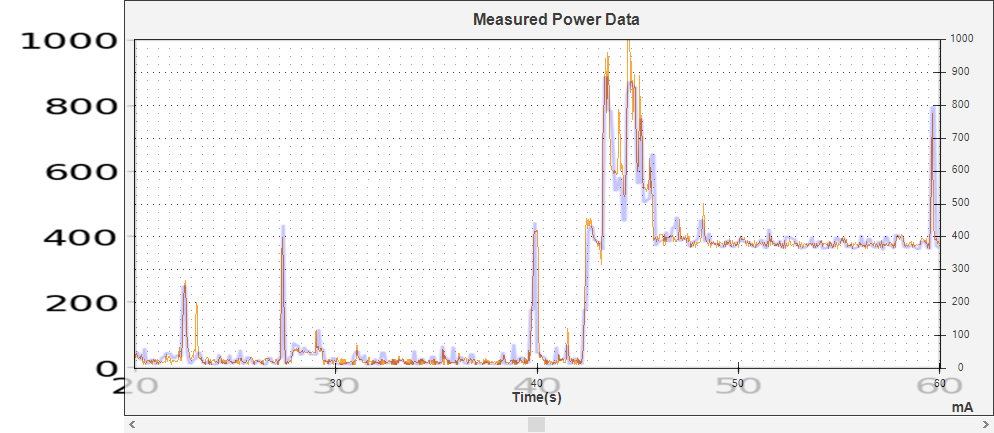
\includegraphics[width=0.45\textwidth]{./figure/1400_base_cpu_idle.png}
	\caption{Stable phone power draw on Nexus 6 during screen-off
          with CPU idle (left half) and 
          during displaying a static image (right half);
         (2) Instantaneous power sensor reading (blue)
         matches with power meter readings (yellow).
        }
	\label{fig:base_current}
        \vspace{-0.2in}
\end{figure}
}

\begin{figure*}[tp]
	\begin{subfigure}[]{0.31\textwidth}
		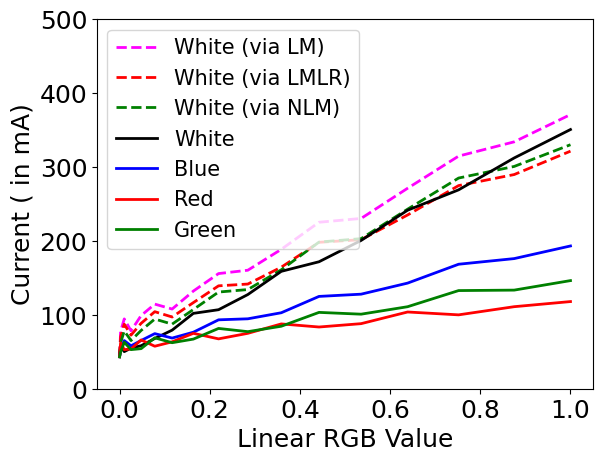
\includegraphics[width=\textwidth]{figure/002_Pixel2_linear_model.png}
		\caption{Pixel 2}
		\label{fig:initial_evaluation_2_n6_w}
	\end{subfigure}
	\hfill
	\begin{subfigure}[]{0.31\textwidth}
		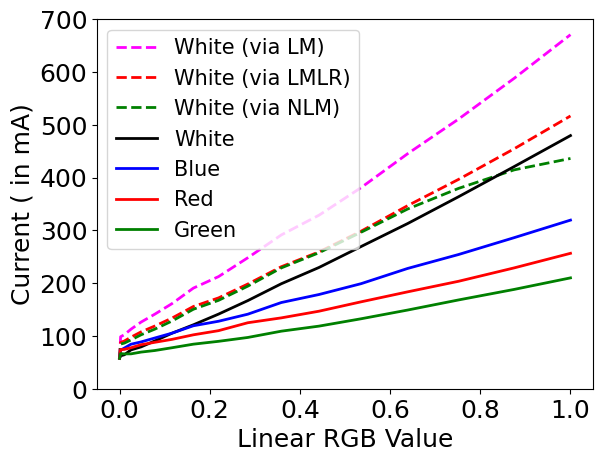
\includegraphics[width=\textwidth]{figure/003_MotoZ3_linear_model.png}
		\caption{Moto Z3}
		\label{fig:initial_evaluation_2_p2_w}
	\end{subfigure}
	\hfill
	\begin{subfigure}[]{0.31\textwidth}
		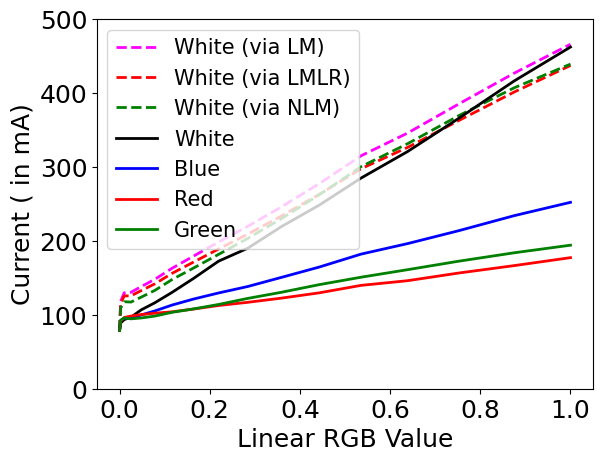
\includegraphics[width=\textwidth]{figure/004_Pixel4_linear_model.png}
		\caption{Pixel 4}
		\label{fig:initial_evaluation_2_z3_w}
	\end{subfigure}
\vspace{-0.1in}
	\caption{OLED display power in displaying one-color images on three phones (with default color mode).
		(LM: linear model as in Eqn.~\ref{eq:linear_equation},
subt		 LMLR: linear model with linear regression, NLM: Non-Linear Model).
}
        \vspace{-0.1in}
        \label{fig:initial_evaluation_2}
\end{figure*}

To accurately measure the phone power draw in our experiments, 
% \eg in displaying a static image, 
we directly connect each of the three
phones to a Monsoon power monitor~\cite{powermonitor}
which has a current sampling rate of 5 KHz.

To facilitate measurements of OLED display power for different colored
pixels, we created a simple Android app that displays a static image
at a time on the screen, while the phone power draw is being measured.
The images used will have the same dimension as the screen, \eg
1920x1080 pixels on Pixel 2.
%    \dtext{Periodically we displayed a black screen where all the pixel
%      values were set to zero and recorded black screen power draw. To get
%      the power draw by colored pixels we subtracted this black screen
%      power from the color static image power draw .}
% To isolate the OLED display power,
%    To isolate the dark screen power, we measure the phone power while
%    the static image is displayed and when the screen is off but CPU is
%    idle (using a wakelock).
First, we measure the CPU idle power 
as the power power draw when the screen is off and the CPU is idle using a wakelock.
Second, we measure the OLED dark screen power 
by displaying a dark screen with all the pixel values set to zero
(during which time the CPU is 99\% idle)
and then subtract the CPU idle power (from Step 1) from the measured phone power.
Finally, to measure the power draw by all the colored pixels,
\ie {$\sum_{i=0}^{n}{P_i}$} in Eqn.~1,
in displaying a staic image (during which time the CPU is also 99\% idle),
 we subtract both the dark
screen power and the CPU idle power
from the phone power measured in displaying the color static image.
%   \forjnl{Figure~\ref{fig:base_current} shows example power meter readings
%   of the two power values.}
\if 0
Since in displaying a static image, the CPU
is 99\% idle and no other phone component is used, the difference
between the two measurements can be attributed to the OLED display power.
\fi

% For easy-of-use,
% our methodology uses built-in power sensor for the actual power measurement.  Since
% the power sensors have relatively coarse resolution, 170ms, 1.4s, and 1.4s, for
% the three phones respectively, we make the app display each image for
% 5 to 10 seconds to gather multiple power sensor readings and use the average as
% the ground truth.


\if 0
Nexus 6, we directly connected the phone to a Monsoon current
Monitor (FTA33D)~\cite{monsoon} to measure the power draw.  For Pixel
2 and Moto Z3 Plus, we used the in-built current sensor to measure the
phone current draw.  To avoid the noise from transient power
fluctuation in displaying a new image, the app displays each image for
5 seconds, during which period the CPU and GPU utilization stays less
than 2\%, and hence the
total power draw consumed by the phone can be attributed to the OLED
display.
\fi

% Since the current sensor reading resolution
% on the two phones are coarse (1.5 seconds), we extend the duration of displaying
% each image to 40 seconds to allow more current
% sensor readings and hence high fidelity in the measured current.

\if 0
\subsection{Pixel Independence}
\label{subsec:basic}

We first validate the two basic assumptions behind
Eqn.~\ref{eq:linear_equation0}.  We make the app display three sequences of
images, each with an increasing percentage of red, green, or blue colored
pixels (with RGB value 255)
respectively, between 0\% and 100\%.  Figure~\ref{fig:basic} shows that (1)
the OLED display draws a non-zero power for dark screen -- this is the
base power $C$, which differ slightly across the 3 phones (Table~\ref{tab:phones}).
\footnote{A major contributor to the base OLED power comes
comes from the touchscreen sensor embedded in the
display~\cite{touchscreenpower}.}
\footnote{In this paper, for power
  measurement we directly report the power using the current drawn, in
  milli-Amperes (mA).  The actual power consumed would be the current
  drawn multiplied by 3.7V, the voltage supply of the battery.}
%
(2) the OLED power draw grows linearly with the percentage
of non-dark pixels of each color -- the
linear curves intersect at RGB value 0.
These results confirm the two
basic assumptions in Eqn.~\ref{eq:linear_equation0}.

%  The same assumptions are made in all previous studies of OLED
%   (\eg~\cite{dong2009current,kim2013runtime}).

\begin{figure}[tp]
        \vspace{-0.1in}
        % \includegraphics[width=0.45\textwidth]{./figure/1500_Horizontal.pdf}
        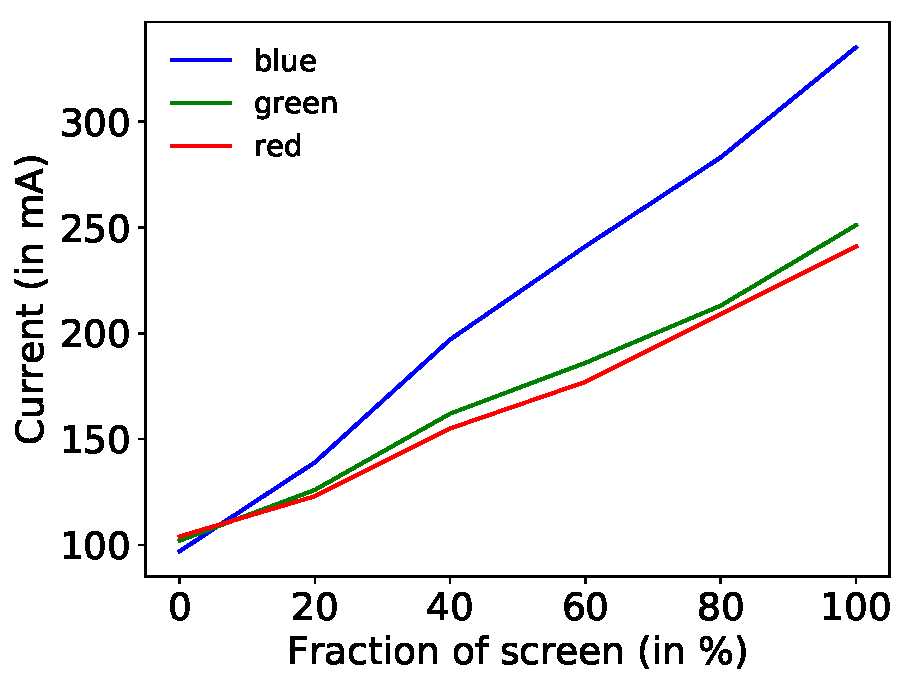
\includegraphics[width=0.30\textwidth]{./figure/1501_Vertical.pdf}
        \vspace{-0.1in}
	\caption{OLED display power under varying percentage of non-dark pixels on Nexus 6.}
        \vspace{-0.1in}
        \label{fig:basic}
\end{figure}

Given that the above two assumptions hold, the remaining challenge
in OLED power modeling
is how to capture the power draw by each pixel $P_i$ as a function of the RGB
values of that pixel ($R_i, G_i,B_i$).

The simplest approach is to measure and tabulate
the power draw of all possible RGB values. This is infeasible
due to the large number of color combinations ($256^3$=16M on modern phone OLED displays).

Since each pixel of OLED display consists of 3 subpixels corresponding
to the three base colors, the most natural approach is to measure the
power draw of each subpixel $f(R_{i})$, $g(G_{i}$, and $h(B_{i})$ as a
function of the color intensity (256$\times$3 measurements), and derive the pixel power
draw for any RGB value as a function of the subpixel power functions:
\begin{equation}
	P_i(R_i, G_i,B_i) = M(f(R_{i}), g(G_{i}), h(B_{i}))
	\label{eq:linear_equation1}
\end{equation}
Subpixel models $f(R_{i})$, $g(G_{i})$ and $h(B_{i})$ can be
trained by displaying monochromatic images on the screen.  For
example, $f(R_{i})$ is obtained as the power in displaying all pixels
in the screen with color ($R_{i}$, 0, 0), minus base power $C$,
and normalized by the total number of pixels.

To gain insight on how to develop the model function $M$,
we next study a few basic properties of the OLED power behavior.

\fi

\subsection{Superposition Property}
\label{subsec:super}

The first question we ask is whether the power draw of the three
subpixels are independent, \ie whether they satisfy the {\em superposition
property} which states that the power consumed by three subpixels are
additive.

\paragraph{Methodology.}
To validate the superposition property, 
we measure the OLED power consumed by
7 monochromatic images containing 3 base colors (red, green, blue),
3 2-channel colors (yellow, magenta and cyan)
and the 3-channel color white, with varying intensities (sRGB values from 0 to 255).

\if 0
\dcomment {
Figures~\ref{fig:initial_evaluation_2}(a)--\ref{fig:initial_evaluation_2}(c)
show the measured OLED display power.
%   for the three base colors and white, and the
%   sum of the power for the three base colors label ``White (via LM)'',
%   on the three phones.
Due to the gamma-correction in sRGB standard,
the subpixel power draw is known to be nonlinear in the sRGB values.
Thus in this paper, we transform the sRGB format into the linear format, known as Linear RGB~\cite{gammaCorrection1} ({$Linear RGB = (sRGB/256)^{2.2}$}),
%  Thus in this paper, we transform the sRGB format into the linear format, known as Linear RGB~\cite{gammaCorrection1},\footnote{$Linear RGB = (sRGB/256)^{2.2}$.}
and plot all OLED power functions w.r.t. Linear RGB values.
Figures~\ref{fig:initial_evaluation_2}(a)--\ref{fig:initial_evaluation_2}(c) show that
(1) the subpixel power draw for the 3 base colors are linear in the Linear RGB values;
(2) the subpixel power draw are not additive -- 
the gap between their sum (without duplicating base power)
and the measured power draw for white
widens with the color intensity,
reaching 2\%, 45\%, and 0.5\% at linear RGB value 1.0 (sRGB value of 255)
for the three phones, respectively.

\forjnl{Figures~\ref{fig:initial_evaluation_2}(d)-\ref{fig:initial_evaluation_2}(f)
  show}

We performed the same analysis for the 2-channel color magenta
(figures not shown due to page limit). Again, we
observe a large deviation between the sum of the power for blue and
red and the actual measurement; the gap widens with the color
intensity, reaching 7\%, 25\%, and 6\% at linear RGB value 1.0 for
the three phones, respectively.  The corresponding gaps are 7\%, 15\%, and 0.8\% for
yellow and 3\%, 17\%, and 2\% for cyan for the three phones.
These results show that
%
{\em subpixel powers are not additive.} The likely reason is that the
  subpixels utilize common driving circuits within the display
  hardware module.
  
CHANGED THIS BECAUSE THE MAXIMUM ERROR IS NOT AT Linear RGB 1.0}
\fi

\paragraph{Findings.}
{
Figures~\ref{fig:initial_evaluation_2}(a)--\ref{fig:initial_evaluation_2}(c)
show the measured OLED display power. Due to the gamma-correction in sRGB standard,
the subpixel power draw is known to be nonlinear in the sRGB values.
Thus in this paper, we transform the sRGB format into the linear format, known as Linear RGB~\cite{gammaCorrection1} ({$Linear RGB = (sRGB/256)^{2.2}$}),
and plot all OLED power functions w.r.t. Linear RGB values.
Figures~\ref{fig:initial_evaluation_2}(a)--\ref{fig:initial_evaluation_2}(c) show that
(1) the subpixel power draw for the 3 base colors are linear in the Linear RGB values;
(2) the subpixel power draw are not additive -- 
the difference between their sum (without duplicating base power)
and the measured power draw for white
varies across the color intensity, reaching
a maximum of 92\%, 66\% and 43\% at
0 (14), 0.04 (59) and 0.01 (25) linear RGB values (sRGB values) for the 3 phones, respectively.
% widens for Moto Z3 with color intensity but decreases for Pixel 2 and Pixel 4.
% widens with the color intensity,
% 1.0 (sRGB value of 255)
% reaching 2\%, 45\%, and 0.5\% at linear RGB value 1.0 (sRGB value of 255)
% for the three phones, respectively.
% \comment{THE GAP IS TOO SMALL FOR P2 and P4. DOES THIS NEEDS TO CHANGE?}

\forjnl{Figures~\ref{fig:initial_evaluation_2}(d)-\ref{fig:initial_evaluation_2}(f)
  show}

We performed the same analysis for the 2-channel color magenta
(figures not shown due to page limit). Again, we
observed a large deviation between the sum of the power individually observed for blue and
red compared to the actual measurement; the gap
% widens with
varies across the color intensity, reaching
55\%, 45\% and 26\% at 0.05 (64), 0.05 (67) and 0.01 (27) linear RGB values (sRGB values)
% at linear RGB value 1.0
for the three phones, respectively.
Simillar gaps are also observed for yellow, \eg of
60\%, 16\% and 18\% at 0.05 (68), 0.10 (91) and 0.02 (43) linear RGB values (sRGB value),
and for cyan, of
44\%, 17\% and 21\% at 0.0 (19), 0.23 (130) and 0.01 (34) linear RGB values (sRGB values),
for the three phones, respectively.
These results show that
%
{\em subpixel powers are not additive.} The likely reason is that the
  subpixels utilize common driving circuits within the display
  hardware module.
}
  
\subsection{Monotonicity Property}
\label{subsec:monoproperty}

We next study whether a more basic property holds in the OLED power
behavior on modern phones.  The {\em monotonicity property} is stated
as follows:

\noindent
{\bf Monotonicity property:}
The OLED pixel power draw for RGB value ($x_1, y_1, z_1$)
is less than that for ($x_2, y_2, z_2$) iff
vector ($x_1, y_1, z_1$) is canonically less than ($x_2, y_2, z_2$),
\ie $x_1 \leq x_2$, $y_1 \leq y_2$, and $z_1 \leq z_2$.

\paragraph{Methodology.}
To validate the monotonicity property, we measure the OLED power draw
in displaying monochromatic images generated by sweeping the 3-D RGB
color space, with each base color intensity varied from 0 to 255 (in
the sRGB space) in steps of 16 (and including value 255) for a total
of 17$^3$ images. We then compare the display power
draw for each pair of adjacent RGB values in the
17$\times$17$\times$17 grid of discretized 3-D color space.



% \begin{figure*}[tp]
% 	\begin{subfigure}[]{0.31\textwidth}
% 		\includegraphics[width=\textwidth]{./figure/275_N6_monotonicity_cube.pdf}
% 		\caption{Nexus 6}
% 		\label{fig:initial_monotonicity_n6_w}
% 	\end{subfigure}
% 	\hfill
% 	\begin{subfigure}[]{0.31\textwidth}
% 		\includegraphics[width=\textwidth]{./figure/277_P2_monotonicity_cube.pdf}
% 		\caption{Pixel 2}
% 		\label{fig:initial_monotonicity_p2_w}
% 	\end{subfigure}
% 	\hfill
% 	\begin{subfigure}[]{0.31\textwidth}
% 		\includegraphics[width=\textwidth]{./figure/276_Z3_monotonicity_cube.pdf}
% 		\caption{Moto Z3}
% 		\label{fig:initial_monotonicity_z3_w}
% 	\end{subfigure}
% 	\caption{The OLED display current showing monotonicity not being
% 		followed on three phones. (Best see in Color)}
% \label{fig:initial_monotonicity}
% \end{figure*}


\paragraph{Findings.}
Interestingly, on all three phones, we found many instances of power
measurements that violate the monotonicity property.  Table~\ref{tab:initial_evaluation_3} lists a few samples for each of the 3
phones, where each row lists the power draw for two color vectors, the
second being canonically larger yet drawing less power than the first.
For example, on Pixel 4, the OLED power draw for RGB value (32, 16, 16) should
be higher than that for (32, 0, 16). Instead,
our measured value for the former, 89mA, 
is 1.09X
lower than that for the later, 97mA.
Since this pattern happens on all three phones,
it is unlikely due to manufacturing defect.
We conjecture\footnote{We could not find any white papers from the OLED vendors
  or the driver source code which are all proprietary.}
that the reasons for the above non-monotonicity behavior
{are two-fold:
(1) there may be OEM-specific color transformation performed
in the hardware composer (Figure~\ref{fig:arch}) that alters the canonical
order of sRGB values;
and
(2) the subpixels utilize
common driving circuits within the display hardware module
differently at different color intensities.
}


\begin{table}[tbp]
	\centering
	\caption{Sample RGB value pairs for which the OLED display
          power violates the monotonicity property.}
        \vspace{-0.1in}
          {\small
          \begin{tabular}{ | l||l|r||l|r| }
		\hline
		Type & Color 1 & Current & Color 2 &  Current \\
                & & (mA) & & (mA) \\
		\hline
                \multicolumn{5}{c }{Pixel 2} \\
		\hline
		1 chl to & ( 176, 0, 0) & 91 & ( 176, 0, 64) & 83 \\
		 2 chl & ( 0, 96, 0) & 79 & ( 0, 96, 16) & 70 \\
		 & ( 0, 0, 16) & 56 & ( 0, 16, 16) & 48 \\
		\hline
		2 chl to & ( 112, 192, 0) & 146 & ( 112, 192, 32) & 131 \\
		 3 chl & ( 112, 0, 80) & 82 & ( 112, 16, 80) & 68 \\
		 & ( 0, 48, 48) & 71 & ( 48, 48, 48) & 53 \\
		\hline
		\multicolumn{5}{c }{Moto Z3} \\
		\hline
		1 chl to & ( 240, 0, 0) & 230 & ( 240, 0, 64) & 225 \\
		 2 chl & ( 0, 224, 0) & 254 & ( 0, 224, 32) & 247 \\
		 & ( 0, 0, 192) & 135 & ( 16, 0, 192) & 133 \\
		\hline
		2 chl to  & ( 240, 240, 0) & 378 & ( 240, 240, 80) & 357 \\
		3 chl & ( 192, 0, 224) & 246 & ( 192, 48, 224) & 220 \\
		 & ( 0, 160, 224) & 242 & ( 64, 160, 224) & 215 \\
		\hline
		\multicolumn{5}{c }{Pixel 4} \\
		\hline
		1 chl to  & ( 80, 0, 0) & 105 & ( 80, 0, 32) & 100 \\
		2 chl & ( 0, 240, 0) & 233 & ( 32, 240, 0) & 230 \\
		 & ( 0, 0, 224) & 173 & ( 16, 0, 224) & 172 \\
		\hline
		2 chl to & ( 128, 16, 0) & 113 & ( 128, 16, 16) & 109 \\
		3 chl  & ( 32, 0, 16) & 97 & ( 32, 16, 16) & 89 \\
		 & ( 0, 176, 192) & 234 & ( 16, 176, 192) & 229 \\
		\hline
	\end{tabular}
         }
	 \label{tab:initial_evaluation_3}
\end{table}

% \begin{figure*}[tp]
% 	\begin{subfigure}[]{0.27\textwidth}
% 		\includegraphics[width=\textwidth]{./figure/401_n6_err.png}
% 		\caption{Nexus 6}
% 	\end{subfigure}
% 	\begin{subfigure}[]{0.27\textwidth}
% 		\includegraphics[width=\textwidth]{./figure/403_p2_err.png}
% 		\caption{Pixel 2 Saturated Color Mode}
% 	\end{subfigure}
% 	\begin{subfigure}[]{0.27\textwidth}
% 		\includegraphics[width=\textwidth]{./figure/402_z3_err.png}
% 		\caption{Moto Z3}
% 	\end{subfigure}
% 	\begin{subfigure}[]{0.10\textwidth}
% 		\includegraphics[width=\textwidth]{./figure/404_err_bar.png}
% 		\caption{Error Bar}
% 	\end{subfigure}
% 
% 	\caption{Prediction error of the linear modeling for the 3-D RGB color space, for all RGB values $(r, g, b)$ where $r, g, b$ are multiples of 16.}
% 	\label{fig:error_wrt_linear}
% \end{figure*}


% We found out how the error varies with respect to the linear model (i.e.
% Equation\ref{eq:linear_equation}) in the color space. The main observation
% is that as we go father away from the (0,0,0) the error increases. In Nexus 6
% we observed that the highest error is observe in the center of the color space.
% This reinforced our conviction that we require a more robust model to cater
% to the OLED display current estimation in mobile phones.

% We start by validating the previous liner OLED current model
% (Eqn~\ref{eq:linear_equation}) via measurements on three phones, Nexus
% 6 (Android Nougat 7.1.1), Pixel 2 (Android 9.0), and Moto Z3 (Anroid
% 9.0), which all have OLED display.
% 
% For Nexus 6, we directly connected the phone to a Monsoon current
% Monitor (FTA33D)~\cite{monsoon}. We created a simple Android app that
% displays one static image at a time on the screen. The images were
% created to have the same dimension as the screen (\eg 2560x1440 pixels
% on Nexus 6). Four series of mono-colored images were displayed,
% corresponding to red, green, blue and white, respectively.
% In each series, consecutive images differ from each other by 10 units of RGB
% value. To avoid the noise from transient current fluctuation in
% displaying a new image, the app displays each image for 5 seconds,
% during which period the CPU and GPU utilization stays less than 1\%
% and the total current consumed by the phone is attributed to the OLED
% display.
% 
% Figure~\ref{fig:initial_evaluation}(a) shows the measured OLED diplay
% current with varying intensities for the 4 mono colors on Nexus 6.
% We make the following observations.
% (1) The blue color  draw far more current than red/green, by 24\% at RGB value of 256;
% (2) The white color only draw marginally more current than blue, by 24\% at RGB value of 256;
% (3) The white color draws far less current than the summation of
% those by red, green and, blue, separately, by 52\% at RGB value of 256, which
% would be the error for the simple linear model.
% 
% We repeated the experiment using Pixel 2 and Moto Z3 Plus using the in-built
% current sensor to measure the phone current draw. Since the current sensor reading resolution
% on the two phones are coarse (1.5 seconds), we extend the duration of displaying
% each image to 40 seconds to allow more current
% sensor readings and hence high fidelity in the measured current.
% 

\subsection{Impact of Brightness Level}
\label{subsec:brightness}

Modern smartphones come with a hardware button or software brightness
slider that allows users to directly adjust the display brightness
level, \eg between 0\% -- 100\%.  We found that {\em brightness level
  adjustment by either scheme does not change frame pixel values
  recorded in the frame buffer}, 
suggesting that some color transformation
caused by the slider brightness level happens after the frame
buffer, \ie in the hardware composer (Figure~\ref{fig:arch}). 
Hence an OLED power model based on the frame pixel values needs to be
adjusted for the display brightness level.
However, our measurements also showed that 
the OLED display power draw does not scale linearly in displaying a same image
with the slider brightness level.

% From reading AOSP source code~\cite{sourcecode:brightness1,sourcecode:brightness2},
We searched the kernel exported hardware info \comment{is this accuract to say?}
and  found that for Android Pie and later vesions, % (\eg Pixel 2 and Moto Z3),
the brightness slider value (0\% to 100\%) is 
%   not linearly correlated with 
transformed to the system screen brightness value (0 to 255),
which can be read from system variable {\small \tt
  /sys/class/leds/lcd-backlight/brightness} on Pixel 2 and Moto Z3
and {{\small \tt /sys/class/backlight
    /panel0-backlight/brightness} on Pixel 4}.  
Second, we experimentally 
% correlated the two brightness levels and 
found that the slider brightness level is mapped 
to the system brightness level via a logarithmic function.
%   Moto Z3 and Pixel 4 by plotting the brightness slider value and 
%   system variable that would lead to the same OLED power draw.
as shown in Figure~\ref{fig:brightnessslider_brightnesslevel}.
Finally, we experimentally confirmed that the OLED display current
scales linearly with the system brightness value in displaying the 7
monochromatic colored images (3 base colors, 3 2-channel colors and
white).

\forjnl{as shown in Figure~\ref{fig:brightnessslider_brightnesslevel}.
}

Our above findings have two implications.
First, when recording a frame as an input to the OLED power model,
we also need to record the system brightness level so that
the output of the pixel value-based power prediction
can be scaled linearly to the system brightness level.
Second, OLED display power at a reduced slider brightness level (\eg 30\%)
actually drains much less power (\eg 9/255 = 3.5\% for Pixel 4 as shown in Figure~\ref{fig:brightnessslider_brightnesslevel}), due to the logarithmic relationship
between the two (slider and system) brightness levels.


\if 0
Modern smartphones come with a hardware button or software brightness
slider that allows users to directly adjust the display brightness
level, \eg between 0\% -- 100\%.  We find that {\em brightness level
  adjustment via either scheme does not change frame pixel values
  recorded in the frame buffer}, suggesting some color transformation
caused by slider brightness level change happens after the frame
buffer, \ie in the hardware composer (Figure~\ref{fig:arch}). 
%  Thus any OLED power model based on the frame pixel values has to
%  explicitly take into account the actual display brightness level.
Furthermore, our measurements show that 
the OLED display power draw in displaying a same image
does not scale linearly with th slider brightness level.

From reading AOSP source code~\cite{sourcecode:brightness1,sourcecode:brightness2},
we found that for Android Pie and later vesions % (\eg Pixel 2 and Moto Z3),
the brightness slider value (between 0\% and 100\%) is 
%   not linearly correlated with 
converted to the system screen brightness value (between 0 and 255)
which can be read from system variable {\small \tt
  /sys/class/leds/lcd-backlight/brightness} on Pixel 2 and Moto Z3
and {{\small \tt /sys/class/backlight
    /panel0-backlight/brightness} on Pixel 4}.  Instead, the mapping
in a logarithmic scale.  The logarithmic scaling follows the XDA
Analysis~\cite{brightness2019} which explains that human eyes observe
noticeable intensity changes in a logarithmic manner.
% the change in the brightness slider (from linear to logarithmic ) is due to the Weber's Law (i.e. the noticeable change.)
%
% This follows the Weber law~\cite{weber} logarithmic property.
%  Earlier with linear scale, it was observed that about 90\% of the brightness was controlled
%  by only left 20\% of the slider~\cite{brightness2019}.
%  Now with the add logarithmic support
%  changes in screen brightness are much more noticeable to human eye
%  when the screen is dark versus when the screen is bright.
We experimentally confirmed this logarithmic brightness level mapping on Pixel 2,
Moto Z3 and Pixel 4 by plotting the brightness slider value and 
system variable that would lead to the same OLED power draw.
\comment{why do we need to do this? cannot we verify by 
reading the two values directly?}
Figure~\ref{fig:brightnessslider_brightnesslevel} shows that
the system brightness value is logarithmically related
with the brightness slider value.
%    To derive the empirical correlation
%    between the brightness slider value and the system variable, we set the variable
%    from 0 to 255 and observed the brightness slider.
%    and the system variable as shown in
%
% for Nexus 6, the two are linearly related whereas
% for Pixel 2 and Moto Z3,
%   The system variables values are 89, 9 \& 11 for 30\% brightness
%   and 136, 22 \& 24 for 50\% brightness
%   for the Nexus 6, Pixel 2 \& Moto Z3 receptivity.
Uncovering this correlation for a given device allows us to calculate
the OLED display power for any brightness slider value.

Finally, we confirmed that
the OLED display current scales linearly with
the system brightness value
% variable {\small \tt /sys/class/leds/lcd-backlight/brightness}
in displaying
%  varied this value in steps of 10 and noted the current drawn separately on
the 7 monochromatic colored images (3 base colors, 3 2-channel colors and white).
The results are omitted due to page limit.
\fi
% We observed that the display current changes linearly,
\forjnl{as shown in Figure~\ref{fig:brightnesss_phones}.
  }

%% To derive the empirical correlation
%% between the brightness slider value and the actual brightness level
%% after color transformation (sent to hardware display), we manually
%% set the system variable /sys/class/leds/lcd-backlight/brightness 0
%% to 255 in increments of 10 and record the display power draw.
%% Similarly, we manually
%% adjust the brightness slider from 0\% to 100\% with increments of 10\%
%% and record the display power draw,
%% in displaying each of the 7 
%% % (3 base colors, 3 2-channel colors and white)
%% monochromatic colored images.
%% We then plot the corresponding values between the slider
%% and the actual brightness level which results in the same display power draw in
%% Figure~\ref{fig:brightnessslider_brightnesslevel}.  We observe
%% indeed that on Nexus 6, the two metrics are lineared related,
%% but on Pixel 2 and Moto Z3, the actual brightness level scales
%% with the logrithmic of the slide values.
%   that at different brightness level is mapped to brightness slider for
%   the phones.  (The orange line is for 30\% and purple like is for 50\%
%   brightness slider levels.)  We also observe that this relationship is
%   not affected by change in the color modes.


\begin{figure}[tb]
	\centering
	\begin{subfigure}[]{0.31\textwidth}
		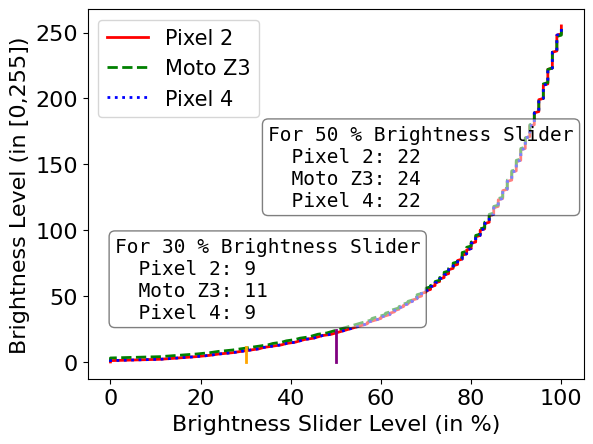
\includegraphics[width=\textwidth]{figure/brightness_curve.png}
	\end{subfigure}
        \vspace{-0.1in}
	\caption{Relationship between the slider brightness level and the system brightness
		value.}
	\label{fig:brightnessslider_brightnesslevel}
\end{figure}

%% With the above unstanding of theslider value, 
%% in Figure~\ref{fig:brightnesss_phones}, we show how the OLED current varies with the
%% actual brightness level.
%% We observe that it follows a linear relationship on all three phones.
%% For Pixel 2 and Moto Z3, we observe that OLED power consumption decreases comparatively
%% more than Nexus 6.
%% In Nexus 6 the brightness slider starts with brightness level 17. This the reason
%% for the sharp drop in the brightness level in Figure~\ref{fig:brightnessslider_brightnesslevel}.
%% Similarly as there the current remain constant for lower value of brightness level
%% in Figure~\ref{fig:brightnesss_phones_n6}.
%% We so conclude that the display power is linearly
%% proportional to the actual brightness level.
%% We use a lookup from brightness slider to the actual brightness level
%% to model their correlation for each phone.

\if 0
\begin{figure*}[tp]
	\begin{subfigure}[]{0.31\textwidth}
		\includegraphics[width=\textwidth]{./figure/a1111_N6_brightness_corrected.pdf}
		\caption{Nexus 6}
		\label{fig:brightnesss_phones_n6}
	\end{subfigure}
	\hfill
	\begin{subfigure}[]{0.31\textwidth}
		\includegraphics[width=\textwidth]{./figure/a1112_P2_brightness_corrected.pdf}
		\caption{Pixel 2}
	\end{subfigure}
	\hfill
	\begin{subfigure}[]{0.31\textwidth}
		\includegraphics[width=\textwidth]{./figure/a1111_Z3_brightness_corrected.pdf}
		\caption{Moto Z3}
	\end{subfigure}
        \vspace{-0.1in}
	\caption{OLED current with varying brightness level for the three phones.
		(The black screen base current is removed.)}
	\label{fig:brightnesss_phones}
\end{figure*}
\fi

\if 0
the OLED power draw are linear in terms of RGB values gamma-corrected
with the brightness level,
as shown in Figures~\ref{fig:brightnesslevel}(c) for Pixel 2,
and captured in Eqn.~(\ref{eq:brigthness_equation_2}:
\begin{equation}
  P_i(R_i, G_i, B_i, Br) = P_i( Br^{2.2}\cdot R_i, Br^{2.2}\cdot G_i, Br^{2.2}\cdot B_i, 1.0)
  \label{eq:brigthness_equation_2}
\end{equation}
where
%$Br$ is the brightness level between 0 to 1 and
$P_i(R_i, G_i, B_i, Br)$ is the pixel power
for RGB value $(R_i, G_i,B_i)$ at brightness level $Br$.
For example, if we
display a white screen with RGB value of (255,255,255) with 80\%
brightness, the display power will be equivalent to having the RGB
value gamma-corrected with the brightness level, \ie (156,156,156)
since $0.8^{2.2}*255=156$. We believe this new
  interpretation of brightness level is a policy change 
that happened starting from {Android O}.
  \fi

  
% \begin{figure}[tp]
% %  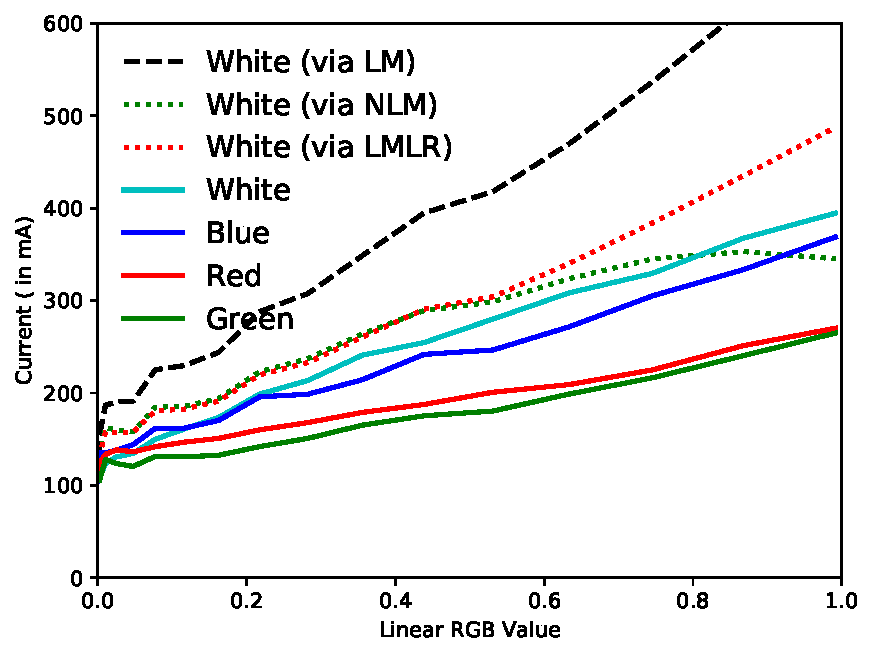
\includegraphics[width=\textwidth]{./figure/240a_n6_standard.pdf}
%         \vspace{-0.1in}
% 	\caption{OLED display power under varying the brightness level.}
%         \vspace{-0.1in}
%         \label{fig:brightnesslevel}
% \end{figure}

% \begin{figure*}[tp]
% 	\begin{subfigure}[]{0.31\textwidth}
% 		\includegraphics[width=\textwidth]{./figure/1100_N6_brightness.pdf}
% 		\caption{Nexus 6}
% 	\end{subfigure}
% 	\begin{subfigure}[]{0.31\textwidth}
% 		\includegraphics[width=\textwidth]{./figure/1122_P2_brightness_with_correction.pdf}
% 		\caption{Pixel 2}
% 	\end{subfigure}
% 	\begin{subfigure}[]{0.31\textwidth}
% 		\includegraphics[width=\textwidth]{./figure/1102_P2_brightness.pdf}
% 		\caption{Pixel 2: with gamma correction}
% 	\end{subfigure}
%         \vspace{-0.1in}
% 	\caption{OLED power draw is linear in the brightness level on Nexus 6 but
%           linear in the brightness-gamma-corrected RGB colors on Pixel 2 and Moto Z3 (not shown).}
% 	\label{fig:brightnesslevel}
% \end{figure*}

% \begin{figure*}[tp]
% 	\begin{subfigure}[]{0.31\textwidth}
% 		\includegraphics[width=\textwidth]{./figure/1100_N6_brightness.pdf}
% 		\caption{Nexus 6}
% 	\end{subfigure}
% 	\begin{subfigure}[]{0.31\textwidth}
% 		\includegraphics[width=\textwidth]{./figure/1102_P2_brightness.pdf}
% 		\caption{Pixel 2}
% 	\end{subfigure}
% 	\begin{subfigure}[]{0.31\textwidth}
% 		\includegraphics[width=\textwidth]{./figure/1101_Z3_brightness.pdf}
% 		\caption{Moto Z3}
% 	\end{subfigure}
%         \vspace{-0.1in}
% 	\caption{OLED power draw is linear in the brightness level on Nexus 6 but
%           nonlinear on Pixel 2 and Moto Z3.}
% 	\label{fig:brightnesslevel}
% \end{figure*}

% To understand the impact of the brightness level on the OLED power
% draw, we measure the OLED power draw by displaying monochromatic
% images of 7 colors: 3 base colors, 3 2-channel colors and white, as
% the display brightness level is adjusted in steps of 20\% using the brightness slider.
% Figures~\ref{fig:brightnessslider_brightnesslevel}(a)-(c) show that
% {\em
% for Nexus 6, the OLED power scales linearly with the brightness level,
% but for Pixel 2  and Moto Z3, the OLED power draw scales linearly
% at low brightness levels but turns exponentially
% at high brightness levels. ??is thisstill true???
% }

%   \comment{
% curve fitting and
%   we found that since Android O, Android interprets 
%   screen brightness level as some intricate color transformation
%   that is not easily described in a simple function.
%   }
%

\subsection{Impact of Color Mode and Color Correction}
\label{subsec:colortransform}

In addition to the brightness level, we found two other forms of color transformation
can happen in recent versions of Android.
First, Android Lollipop introduced 
{\em color correction} for visually impaired users~\cite{colorcorrection}.
% , which also uses HardwareComposer to change the color actually displayed.
%  Color correction comes with 3 modes: Deuteranomaly (red-green),
Second, Android 8.1 Oreo added templates for adding new {\em color modes}.
%with the help of HardwareComposer2~\cite{colormode}
%  which uses HardwareComposer2~\cite{colormode} to perform color
%  transformation to change the color displayed.
% It requires factory calibration data, stored in the device, to adjust variation in manufacturing.
OEMs can use this template mechanism to display vibrant colors by utilizing
the wide color gamut.
\forjnl{For example, Pixel 2 phones provide 3 color modes:
Natural, Boosted (default) and Saturated,
and Moto Z3 phones come with 2 color modes, Standard and Vibrant (Default), and
Vibrant has 3
variations, namely, Warm, Neutral (Default) and Cool.
Figure~\ref{fig:initial_evaluation_color_mode} in Appendix A2
shows that the OLED power draw in displaying the same monochromatic images 
for non-default color modes on Pixel 2 and Moto Z3 differ from
those in Figure~\ref{fig:initial_evaluation_2}.
}
%  Protanomaly (red-green), and Tritanomaly (blue-yellow).

Both color change features are implemented by passing a color
matrix~\cite{colormatrix} to the hardware composer, which performs the
color transformation on the frame pixels before sending them to the
display. In doing so,
they alter the OLED power draw without changing
the frame buffer recorded, similarly as with brightness level adjustment.
{For example, our measurments have shown (results omitted due to page limit)
  that on Pixel 2, displaying the same
  white-color image under Natural and Saturated Color Modes
draws 2.6\% and 4.9\% more power than the default color mode.
}
% cannot catch such color-transformed pixels sent to the display, and hence
Hence, {\em OLED power models using frame buffer as input need to be derived
for each color mode or correction.}



\section{Limitation of Previous Models}
\label{sec:non_linear}

Since directly measuring the power draw of every pixel color is too
costly (\eg it would take $256^3$$\times$10 seconds or 5.3 years following
our methodology of displaying each image for 5 seconds), power modeling has been proposed to estimate the OLED
power draw of any pixel color based on measurements of a few pixel colors.

% additive model
% linear regression
% non-linear modeling

% Linear (r+g+b)
% linear (*r + *g + * b +(r+g+b)) 
% Kim is some hack - cannot reproduce

\paragraph{Simple linear model.}
\label{subsec:LM}
Dong~\etal~\cite{dong2009current} proposed one of the first pixel-level OLED current models,
which models the pixel power draw as the simple sum of
those of subpixels:
\begin{equation}
	P_i(R_i, G_i,B_i) = f(R_{i}) + g(G_{i}) + h(B_{i})
	\label{eq:linear_equation}
\end{equation}
and showed that the model  achieves an average 
error of 1\% in
displaying 300 benchmark images on an external OLED QVGA display
module with a standard 16-bit (5, 6, 5) RGB setting.
%
The simple linear model (denoted as LM) cannot model the OLED power on modern phones
which violate the superposition property.
%as discussed in \S\ref{subsec:super}.

%   We note the model of interest in this paper
%   is that of the pixel power draw as a function of the power
%   draw of subpixels, which we denote this as {\em pixel power model}.
%   The individual subpixel power draw 
%   $f(R_{i})$, $g(G_{i}$, and $h(B_{i})$ are known to be linear with respect to
%   the color value $R_{i}, G_i, B_i$ after gamma correction~\cite{???}.

%  The above property pertains to power behavior of subpixels within a pixel.
%  Since the individual subpixel power draw functions
%  $f(R_{i})$, $g(G_{i}$, and $h(B_{i})$ are known to be monotonically increasing with respect to
%  the color values $R_{i}, G_i, B_i$~\cite{???}, any linear pixel power model
%  also posses the following property:

%  \begin{itemize}
%  \item {\bf Monotonicity:} The higher the RGB values, the higher the pixel power draw.
%    For example, RGB values of (32, 32, 32) will result in higher pixel power draw than
%    RGB values of (32, 32, 0).
%  \end{itemize}


\paragraph{Adding Linear Regression.}
\label{subsec:LMLR}
Violation of the superposition property has been observed
previously~\cite{mittal2012empowering,kim2013runtime}
and suggests the power draw of three subpixels
are not independent.
The simplest idea to accommodate the dependence is to introduce liner regression,
as suggested by Kim~\etal~\cite{kim2013runtime},
%  performed one of the first
%  validations of the simple OLED power model (Eqn.~\ref{eq:linear_equation}
%  on smartphones and also
\forjnl{, who were among the first to discover that the OLED power draw violates the
  superposition property.}
who showed extending the
simple summation into a linear formula with the coefficients dervied
via linear regression reduces the average error from 8.0\% to 1.4\% on
Galaxy S3 for a set of screen images of 10 Android apps.

\if 0
\begin{equation}
P_i = Br\cdot(f(R_{i}) + g(G_{i}) + h(B_{i}) + e(R_{i},G_{i},B_{i}))
\label{eq:linear_equation2}
\end{equation}
\noindent
where $Br$ is the normalized brightness level and $e(R,G,B)= a(R+G+B)
+ b$, is a linear regression term with empirically estimated
coefficients. \
\fi

\if 0
To validate if linear regression can capture the OLED power behavior
on the 3 modern phones in our experiments, we derive linear
regressions on the power draw of the 3 base colors to fit the power
draw of the 3 2-channel colors (yellow, magenta and cyan) and 1 3-channel color (white).
Eqn.~\ref{eq:linear_independent} shows the coefficients of the linear
regressions.  We see that the coefficients of the four linear
regressions differ significantly, suggesting the dependence among the
power draw of subpixel cannot be easily captured with a single linear
model from linear regression.

\begin{subequations}
\begin{align}
	&\begin{bmatrix}
	    P_{y} \\
	    P_{m} \\
	    P_{c} \\
	    P_{w}
	\end{bmatrix}
	=
	\begin{bmatrix}
		T
	\end{bmatrix}
	\begin{bmatrix}
	    P_{r} &
	    P_{g} &
	    P_{b}
	\end{bmatrix}^T
	\\
	&\begin{bmatrix}
		T
	\end{bmatrix}
	=
	\mbox{Coefficients from linear regression to fit 4 colors} \nonumber
	\\
	&Nexus 6: \nonumber
	\\
	&\begin{bmatrix}
	     1.091 &      0.607 &      0.000 \\
	     1.539 &      0.000 &      0.015 \\
	     0.000 &      1.982 &      0.244 \\
	     0.621 &      1.586 &      0.029
	\end{bmatrix}
	\\
	&Moto Z3:  \nonumber
	\\
	&\begin{bmatrix}
	     1.103 &      0.439 &      0.000 \\
	     0.247 &      0.000 &      1.226 \\
	     0.000 &      0.023 &      1.338 \\
	     0.942 &      0.693 &      0.327
	\end{bmatrix}
	\\
	&Pixel 2:  \nonumber
	\\
	&\begin{bmatrix}
	     0.544 &      1.489 &      0.000 \\
	     0.638 &      0.000 &      1.000 \\
	     0.000 &      1.193 &      0.739 \\
	    -0.201 &      4.125 &     -0.401
	\end{bmatrix}
\end{align}
	\label{eq:linear_independent}
\end{subequations}
\fi

\forjnl{Figure~\ref{fig:initial_evaluation_2} shows that the
OLED display power for based colors red, green, and blue ($f(R_{i})$,
$g(G_{i})$, and $h(B_{i})$) and white and magenta are all linear w.r.t.
the linear RGB value.  Therefore, it is conceivable to derive a linear
regression of $f(R_{i})$, $g(G_{i})$, and $h(B_{i})$ to match well with
the OLED power draw of any single color, \eg white.
}

Since the power model should model the pixel power draw for
any combinations of RGB values, to assess the feasibility of the above model, we 
derived linear regression of $f(R_{i})$, $g(G_{i})$, and $h(B_{i})$ 
to fit the power draw of 4 colors, yellow, magenta and cyan, and white,
as the intensity varies from 0 to 255\footnote{We use 4-color monochromatic images to train these
  models because that they cover the sRGB space and gives us 256$\times$4=1024 equations.
  Training the models using real images may not cover the entire color space or provide
  enough diversity.}. The derived models
for the 3 phones are:

\hspace{-0.1in}
{\small
  \begin{eqnarray}
%\begin{align}
	P_i^{Pixel 2} = 0.700*f(R_i) + 0.928*g(G_i) + 0.868*h(B_i) \\
	P_i^{Moto Z3} = 0.665*f(R_i) + 0.928*g(G_i) + 0.708*h(B_i) \\
	P_i^{Pixel 4} = 0.779*f(R_i) + 1.047*g(G_i) + 0.929*h(B_i)
%\end{align}
	\label{eq:linear_model_linear_regression}
  \end{eqnarray}
}
\noindent
The models do not have constant terms because the base power is
already accounted in Eqn.~\ref{eq:linear_equation0}.

We then plot the predicted power with the new models for white in
Figure~\ref{fig:initial_evaluation_2}, labeled as LMLR.  We see that the new model
improves the accuracy of the simple superposition model LM, but still
incurs an average (over linear RGB values)
prediction error of 13\%, 9\%, and 8\% for white
(and 13\%, 14\%, and 7\% for magenta which are not shown) on the 3 phones, respectively.

A second reason that such linear regression based models are inaccurate
is that they are linear in the subpixel powers (with positive coefficients), and hence still
assume the monotonicity property which does not hold as shown
in \S\ref{subsec:monoproperty}.

% \begin{equation}
% 	\begin{bmatrix}
% 	    y \\
% 	    m \\
% 	    c \\
% 	    w
% 	\end{bmatrix}
% 	=
% 	\begin{bmatrix}
% 	     1.091 &      0.607 &      0.000 \\
% 	     1.539 &      0.000 &      0.015 \\
% 	     0.000 &      1.982 &      0.244 \\
% 	     0.621 &      1.586 &      0.029
% 	\end{bmatrix}
% 	\begin{bmatrix}
% 	    r \\
% 	    g \\
% 	    b
% 	\end{bmatrix}
% 	\label{eq:linear_independent}
% \end{equation}
% 
% \begin{equation}
% 	\begin{bmatrix}
% 	    y \\
% 	    m \\
% 	    c \\
% 	    w
% 	\end{bmatrix}
% 	=
% 	\begin{bmatrix}
% 	     1.103 &      0.439 &      0.000 \\
% 	     0.247 &      0.000 &      1.226 \\
% 	     0.000 &      0.023 &      1.338 \\
% 	     0.942 &      0.693 &      0.327
% 	\end{bmatrix}
% 	\begin{bmatrix}
% 	    r \\
% 	    g \\
% 	    b
% 	\end{bmatrix}
% \end{equation}
% 
% \begin{equation}
% 	\begin{bmatrix}
% 	    y \\
% 	    m \\
% 	    c \\
% 	    w
% 	\end{bmatrix}
% 	=
% 	\begin{bmatrix}
% 	     0.544 &      1.489 &      0.000 \\
% 	     0.638 &      0.000 &      1.000 \\
% 	     0.000 &      1.193 &      0.739 \\
% 	    -0.201 &      4.125 &     -0.401
% 	\end{bmatrix}
% 	\begin{bmatrix}
% 	    r \\
% 	    g \\
% 	    b
% 	\end{bmatrix}
% \end{equation}


\paragraph{Using non-linear models.}
\label{subsec:nonlinear}
Another measurement study~\cite{park2015accurate} on an external
AMOLED module
% also
suggested % subpixels are not independent and proposed
adding non-linear terms, in particular, pairwise two-color
coupling terms, to reduce the modeling error of linear models.


\if 0
Eqn.\ref{eq:linear_dependent} the resulting coefficients.

\begin{subequations}
\begin{align}
	&\begin{bmatrix}
	    P_{y} \\
	    P_{m} \\
	    P_{c} \\
	    P_{w}
	\end{bmatrix}
	=
	\begin{bmatrix}
		T
	\end{bmatrix}
	\begin{bmatrix}
	    P_{r} 	       &
	    P_{g} 	       &
	    P_{b} 	       &
	    P_{r}*P_{g}        &
	    P_{r}*P_{b}        &
	    P_{b}*P_{g}        &
	    P_{r}*P_{g}*P_{b}
	\end{bmatrix}^T
	\\
	&\begin{bmatrix}
		T
	\end{bmatrix}
	=
		Linear Dependent Transformation \nonumber
	\\
	&Nexus 6: \nonumber
	\\
	&\begin{bmatrix}
	      1.11 &       0.57 &       0.00 &       0.00 &       0.00 &       0.00 &       0.00 \\
	      1.20 &       0.00 &      -0.16 &       0.00 &       0.00 &       0.00 &       0.00 \\
	      0.00 &       2.70 &       0.21 &       0.00 &       0.00 &      -0.00 &       0.00 \\
	      1.37 &       1.97 &      -1.53 &      -0.04 &       0.03 &       0.00 &      -0.00
	\end{bmatrix}
	\\
	&Moto Z3: \nonumber
	\\
	&\begin{bmatrix}
	      1.14 &       0.18 &       0.00 &       0.00 &       0.00 &       0.00 &       0.00 \\
	     -0.41 &       0.00 &       1.27 &       0.00 &       0.00 &       0.00 &       0.00 \\
	      0.00 &      -0.17 &       1.37 &       0.00 &       0.00 &       0.00 &       0.00 \\
	      0.98 &       2.34 &      -1.07 &      -0.04 &       0.01 &       0.02 &       0.00
	\end{bmatrix}
	\\
	&Pixel 2: \nonumber
	\\
	&\begin{bmatrix}
	      0.64 &       1.29 &       0.00 &       0.00 &       0.00 &       0.00 &       0.00 \\
	     -0.04 &       0.00 &       1.12 &       0.00 &       0.01 &       0.00 &       0.00 \\
	      0.00 &       1.76 &       0.49 &       0.00 &       0.00 &      -0.00 &       0.00 \\
	     -1.41 &       3.25 &       0.34 &      -0.13 &       0.09 &      -0.02 &       0.00
	\end{bmatrix}
\end{align}
	\label{eq:linear_dependent}
\end{subequations}
\fi

  \if 0
  &\begin{bmatrix}
	    P_{y} \\
	    P_{m} \\
	    P_{c} \\
	    P_{w}
	\end{bmatrix}
  \fi

We experimented with such a non-linear model (denoted as NLM),
by adding pairwise two-color
coupling terms and a three-color coupling term,
and applying linear regression to derive the coefficients
of the resulting polynomial model to fit the power draw
of the same 4 colors, yellow, magenta and cyan, and white:

\hspace{-0.2in}
  {\small
  \begin{eqnarray}
  P&=&V\cdot [ 
	    f(Ri)\mbox{\hspace{0.07in}}
	    g(G_i)\mbox{\hspace{0.07in}}
	    h(B_i)\mbox{\hspace{0.07in}}
	    f(Ri)\cdot g(G_i)\mbox{\hspace{0.07in}}\\
&&	    f(Ri)\cdot h(B_i)\mbox{\hspace{0.07in}}
	    g(G_i)\cdot h(B_i)\mbox{\hspace{0.07in}}
	    f(Ri)\cdot g(G_i)\cdot h(B_i)
  ]^T
	\nonumber \\
%V=	\mbox{Coefficients from linear regression to fit 4 colors} \nonumber \\
        V_{Pixel 2} &=& \lbrack 0.33\mbox{\hspace{0.07in}}
        0.61\mbox{\hspace{0.07in}}
        0.65\mbox{\hspace{0.07in}}
        0.01\mbox{\hspace{0.07in}}
        0.01\mbox{\hspace{0.07in}}
        0.01\mbox{\hspace{0.07in}}
        -0.00 \rbrack   \nonumber \\
        V_{Moto Z3} &=& \lbrack 0.42\mbox{\hspace{0.07in}}
        1.22\mbox{\hspace{0.07in}}
        0.53\mbox{\hspace{0.07in}}
        0.00\mbox{\hspace{0.07in}}
        0.00\mbox{\hspace{0.07in}}
        0.00\mbox{\hspace{0.07in}}  -0.00\rbrack \nonumber  \\
        V_{Pixel 4} &=& \lbrack 0.29\mbox{\hspace{0.07in}}
        0.93\mbox{\hspace{0.07in}}
        0.86\mbox{\hspace{0.07in}}
        0.01\mbox{\hspace{0.07in}}
        0.01\mbox{\hspace{0.07in}}
        0.00\mbox{\hspace{0.07in}}
        -0.00 \rbrack \nonumber 
\end{eqnarray}
}
\noindent
\comment{I wonder why the coefficients for the 1st 3 terms so different from the LMLR model}
Note that the coefficients for the nonlinear terms are very small (close to but not equal zero)
due to the larger magnitudes of the nonlinear terms.
We again plot the predicted power using the derived non-linear model
for magenta and white for varying intensities in
Figure~\ref{fig:initial_evaluation_2}, labeled as NLM.
We see that compared to LMLR, the NLM model 
sometimes over-predicts (for small linear RGB values)
and sometimes under-predicts (for large linear RGB values) the power for the
white color, but overall exhibits similar accuracy as the
LMLR models.
{The average prediction error is
10\%, 10\%, and 7\% for white
and 3\%, 4\%, and 3\% for magenta on the 3 phones, respectively.
}

\if 0
{Again, since the coefficients of all terms are positive,}
the predicted power of these NLM models will exhibit the monotonicity property
with increasing RGB values, which are not met in the measured power values.
\fi

% \begin{equation}
% 	\begin{bmatrix}
% 	    y \\
% 	    m \\
% 	    c \\
% 	    w
% 	\end{bmatrix}
% 	=
% 	\begin{bmatrix}
% 	      1.11 &       0.57 &       0.00 &       0.00 &       0.00 &       0.00 &       0.00 \\
% 	      1.20 &       0.00 &      -0.16 &       0.00 &       0.00 &       0.00 &       0.00 \\
% 	      0.00 &       2.70 &       0.21 &       0.00 &       0.00 &      -0.00 &       0.00 \\
% 	      1.37 &       1.97 &      -1.53 &      -0.04 &       0.03 &       0.00 &      -0.00
% 	\end{bmatrix}
% 	\begin{bmatrix}
% 	    r \\
% 	    g \\
% 	    b \\
% 	    r*g \\
% 	    r*b \\
% 	    b*g \\
% 	    r*g*b
% 	\end{bmatrix}
% 	\label{eq:linear_dependent}
% \end{equation}
% 
% \begin{equation}
% 	\begin{bmatrix}
% 	    y \\
% 	    m \\
% 	    c \\
% 	    w
% 	\end{bmatrix}
% 	=
% 	\begin{bmatrix}
% 	      1.14 &       0.18 &       0.00 &       0.00 &       0.00 &       0.00 &       0.00 \\
% 	     -0.41 &       0.00 &       1.27 &       0.00 &       0.00 &       0.00 &       0.00 \\
% 	      0.00 &      -0.17 &       1.37 &       0.00 &       0.00 &       0.00 &       0.00 \\
% 	      0.98 &       2.34 &      -1.07 &      -0.04 &       0.01 &       0.02 &       0.00
% 	\end{bmatrix}
% 	\begin{bmatrix}
% 	    r \\
% 	    g \\
% 	    b \\
% 	    r*g \\
% 	    r*b \\
% 	    b*g \\
% 	    r*g*b
% 	\end{bmatrix}
% \end{equation}
% 
% \begin{equation}
% 	\begin{bmatrix}
% 	    y \\
% 	    m \\
% 	    c \\
% 	    w
% 	\end{bmatrix}
% 	=
% 	\begin{bmatrix}
% 	      0.64 &       1.29 &       0.00 &       0.00 &       0.00 &       0.00 &       0.00 \\
% 	     -0.04 &       0.00 &       1.12 &       0.00 &       0.01 &       0.00 &       0.00 \\
% 	      0.00 &       1.76 &       0.49 &       0.00 &       0.00 &      -0.00 &       0.00 \\
% 	     -1.41 &       3.25 &       0.34 &      -0.13 &       0.09 &      -0.02 &       0.00
% 	\end{bmatrix}
% 	\begin{bmatrix}
% 	    r \\
% 	    g \\
% 	    b \\
% 	    r*g \\
% 	    r*b \\
% 	    b*g \\
% 	    r*g*b
% 	\end{bmatrix}
% \end{equation}

\if 0
Thirdly, we tried to fit into a higher order polynomial. We show here the linear
regression output that we got from a 2nd order polynomial. But unfortunately we
can not find a polynomial we can accurately describe the relationship between
the display current and the individual component current.
We conclude that we can't model the display current by curve fitting techniques
for the entire color space.

\begin{subequations}
\begin{align}
	&\begin{bmatrix}
	    P_{y} \\
	    P_{m} \\
	    P_{c} \\
	    P_{w}
	\end{bmatrix}
	=
	\begin{bmatrix}
		T
	\end{bmatrix}
	\begin{bmatrix}
	    P_{r^2}            &
	    P_{g^2}            &
	    P_{b^2}            &
	    P_{r}              &
	    P_{g}              &
	    P_{b}              &
	    P_{r}*P_{g}        &
	    P_{r}*P_{b}        &
	    P_{b}*P_{g}        &
	    P_{r}*P_{g}*P_{b}
	\end{bmatrix}
	\\
	&\begin{bmatrix}
		T
	\end{bmatrix}
	=
		Non-Linear Dependent Transformation Matrix \nonumber
	\\
	&Nexus 6: \nonumber
	\\
	&\begin{bmatrix}
	     -0.02 &      -0.04 &       0.00 &       1.50 &      -0.10 &       0.00 &       0.06 &       0.00 &       0.00 &       0.00 \\
	      0.02 &       0.00 &      -0.01 &      -1.36 &       0.00 &       1.96 &       0.00 &       0.00 &       0.00 &       0.00 \\
	      0.00 &      -0.01 &      -0.01 &       0.00 &       0.53 &       1.23 &       0.00 &       0.00 &       0.02 &       0.00 \\
	      0.34 &      -0.16 &      -0.00 &      -6.82 &      -1.03 &       6.90 &      -0.24 &      -0.32 &       0.36 &      -0.00
	\end{bmatrix}
	\\
	&Moto Z3: \nonumber
	\\
	&\begin{bmatrix}
	     -0.00 &      -0.02 &       0.00 &       0.51 &       1.29 &       0.00 &       0.02 &       0.00 &       0.00 &       0.00 \\
	     -0.04 &       0.00 &      -0.01 &       1.08 &       0.00 &      -0.05 &       0.00 &       0.05 &       0.00 &       0.00 \\
	      0.00 &       0.00 &       0.01 &       0.00 &       0.85 &       0.78 &       0.00 &       0.00 &      -0.01 &       0.00 \\
	      0.05 &      -0.00 &       0.09 &       1.06 &       2.60 &      -1.48 &       0.06 &      -0.13 &      -0.07 &       0.00
	\end{bmatrix}
	\\
	&Pixel 2: \nonumber
	\\
	&\begin{bmatrix}
	     -0.04 &      -0.08 &       0.00 &       0.46 &       1.60 &       0.00 &       0.11 &       0.00 &       0.00 &       0.00 \\
	     -0.09 &       0.00 &      -0.07 &      -2.05 &       0.00 &       2.77 &       0.00 &       0.17 &       0.00 &       0.00 \\
	      0.00 &      -0.08 &      -0.02 &       0.00 &       1.06 &       0.77 &       0.00 &       0.00 &       0.09 &       0.00 \\
	      0.24 &       0.82 &       0.37 &      -1.39 &       4.65 &      -0.69 &      -0.09 &      -0.27 &      -0.90 &      -0.00
	\end{bmatrix}
\end{align}
	\label{eq:nonlinear_dependent}
\end{subequations}
\fi

% \begin{equation}
% 	\resizebox{\columnwidth}{!}{$
% 	\begin{bmatrix}
% 	    y \\
% 	    m \\
% 	    c \\
% 	    w
% 	\end{bmatrix}
% 	=
% 	\begin{bmatrix}
% 	     -0.02 &      -0.04 &       0.00 &       1.50 &      -0.10 &       0.00 &       0.06 &       0.00 &       0.00 &       0.00 \\
% 	      0.02 &       0.00 &      -0.01 &      -1.36 &       0.00 &       1.96 &       0.00 &       0.00 &       0.00 &       0.00 \\
% 	      0.00 &      -0.01 &      -0.01 &       0.00 &       0.53 &       1.23 &       0.00 &       0.00 &       0.02 &       0.00 \\
% 	      0.34 &      -0.16 &      -0.00 &      -6.82 &      -1.03 &       6.90 &      -0.24 &      -0.32 &       0.36 &      -0.00
% 	\end{bmatrix}
% 	\begin{bmatrix}
% 	    r^2 \\
% 	    g^2 \\
% 	    b^2 \\
% 	    r \\
% 	    g \\
% 	    b \\
% 	    r*g \\
% 	    r*b \\
% 	    b*g \\
% 	    r*g*b
% 	\end{bmatrix}
% 	$}
% 	\label{eq:nonlinear_dependent}
% \end{equation}
% 
% \begin{equation}
% 	\resizebox{\columnwidth}{!}{$
% 	\begin{bmatrix}
% 	    y \\
% 	    m \\
% 	    c \\
% 	    w
% 	\end{bmatrix}
% 	\\
% 	=
% 	\begin{bmatrix}
% 	     -0.00 &      -0.02 &       0.00 &       0.51 &       1.29 &       0.00 &       0.02 &       0.00 &       0.00 &       0.00 \\
% 	     -0.04 &       0.00 &      -0.01 &       1.08 &       0.00 &      -0.05 &       0.00 &       0.05 &       0.00 &       0.00 \\
% 	      0.00 &       0.00 &       0.01 &       0.00 &       0.85 &       0.78 &       0.00 &       0.00 &      -0.01 &       0.00 \\
% 	      0.05 &      -0.00 &       0.09 &       1.06 &       2.60 &      -1.48 &       0.06 &      -0.13 &      -0.07 &       0.00
% 	\end{bmatrix}
% 	\\
% 	\begin{bmatrix}
% 	    r^2 \\
% 	    g^2 \\
% 	    b^2 \\
% 	    r \\
% 	    g \\
% 	    b \\
% 	    r*g \\
% 	    r*b \\
% 	    b*g \\
% 	    r*g*b
% 	\end{bmatrix}
% 	$}
% \end{equation}
% 
% \begin{equation}
% 	\resizebox{\columnwidth}{!}{$
% 	\begin{bmatrix}
% 	    y \\
% 	    m \\
% 	    c \\
% 	    w
% 	\end{bmatrix}
% 	=
% 	\begin{bmatrix}
% 	     -0.04 &      -0.08 &       0.00 &       0.46 &       1.60 &       0.00 &       0.11 &       0.00 &       0.00 &       0.00 \\
% 	     -0.09 &       0.00 &      -0.07 &      -2.05 &       0.00 &       2.77 &       0.00 &       0.17 &       0.00 &       0.00 \\
% 	      0.00 &      -0.08 &      -0.02 &       0.00 &       1.06 &       0.77 &       0.00 &       0.00 &       0.09 &       0.00 \\
% 	      0.24 &       0.82 &       0.37 &      -1.39 &       4.65 &      -0.69 &      -0.09 &      -0.27 &      -0.90 &      -0.00
% 	\end{bmatrix}
% 	\begin{bmatrix}
% 	    r^2 \\
% 	    g^2 \\
% 	    b^2 \\
% 	    r \\
% 	    g \\
% 	    b \\
% 	    r*g \\
% 	    r*b \\
% 	    b*g \\
% 	    r*g*b
% 	\end{bmatrix}
% 	$}
% \end{equation}


\begin{figure}[tp]
	\begin{subfigure}[]{0.25\columnwidth}
		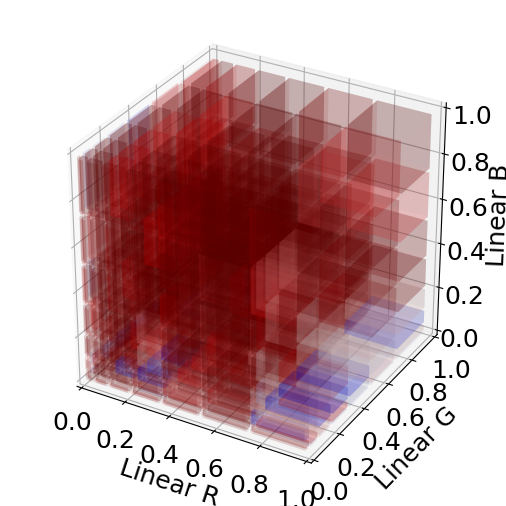
\includegraphics[width=\linewidth]{figure/002_Pixel2_error_cuve.png}
		\caption{Pixel 2}
	\end{subfigure}
	\hfill
	\begin{subfigure}[]{0.25\columnwidth}
		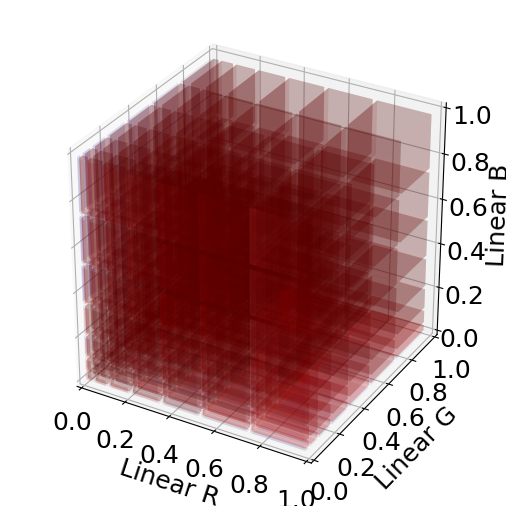
\includegraphics[width=\linewidth]{figure/003_MotoZ3_error_cuve.png}
		\caption{Moto Z3}
	\end{subfigure}
	\hfill
	\begin{subfigure}[]{0.25\columnwidth}
		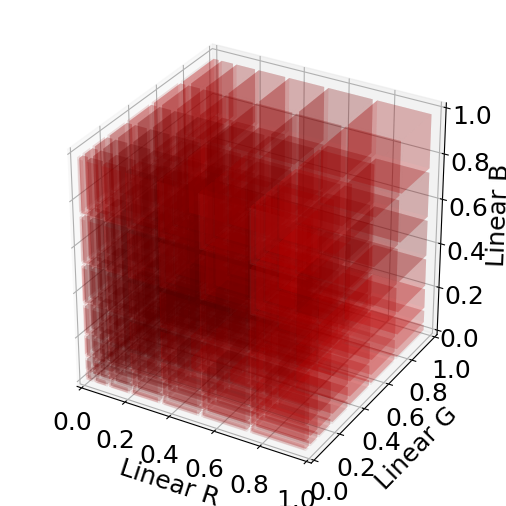
\includegraphics[width=\linewidth]{figure/004_Pixel4_error_cuve.png}
		\caption{Pixel 4}
	\end{subfigure}
	\hfill
	\begin{subfigure}[]{0.15\columnwidth}
		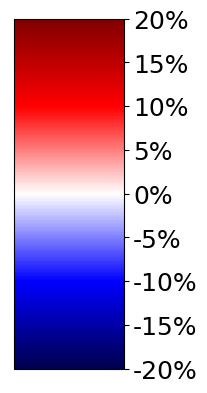
\includegraphics[width=0.8\linewidth]{figure/004_error_bar.png}
		% \caption{Error Bar}
	\end{subfigure}
        \vspace{-0.1in}
	\caption{Prediction error of the LMLR model in the linear RGB
          color space, for all sRGB values $(r, g, b)$, $r, g, b$
          are multiples of 16.}
        \vspace{-0.2in}
	\label{fig:error_wrt_linear}
\end{figure}


\paragraph{Model error across the color space.}
%  
% {what model did we use for this?}
Since prior-art models cannot even approximate 4 monochromatic
colors well, we can expect that they will have high prediction errors
in the entire 3-D color space. We further measured
the prediction error of the {LMLR} model at all RGB values of $(x, y,
z)$ where $x, y, z$ spans all multiples of 16. The results, shown
in Figure~\ref{fig:error_wrt_linear}, confirm that the {LMLR} model
exhibits high error across the color space on all three phones,
with a mean absolute prediction error of 6.90\%, 10.35\%, 7.10\%,
and 90th percentile absolute error of  15.65\%, 22.07\%, 16.19\%,
respectively, for the three phones.
Interestingly, the error is lower on Pixel 2 and Pixel 4, which can be explained
by their least violation of superposition property as shown in Figure~\ref{fig:initial_evaluation_2}.
Similarly, we observed that the {NLM} model also
exhibits high error across the color space on all three phones,
with a mean absolute prediction error of 6.79\%, 12.94\%, 6.02\%,
and 90th percentile absolute error of  15.45\%, 28.75\%, 13.38\%,
respectively, for the three phones.
% \comment{
% with a mean absolute prediction error of ???\%, ??\%, and ??\%,
% and 90th percentile absolute error of  ???\%, ??\%, and ??\%,
% respectively.
% }
% Interestingly, the error is lower on Pixel 2, which can be explained
% by its least violation of superposition property shown in Figure~\ref{fig:initial_evaluation_2}.

% \comment{can we add these error numbers for NLM?}

\section{A New OLED Power Model}
\label{sec:newmodel}

In this section, we present a practical OLED pixel power model that
is more accurate than prior arts and robust to device diversities.

\begin{figure*}[tp]
	\hfill
	\begin{subfigure}[]{0.28\textwidth}
		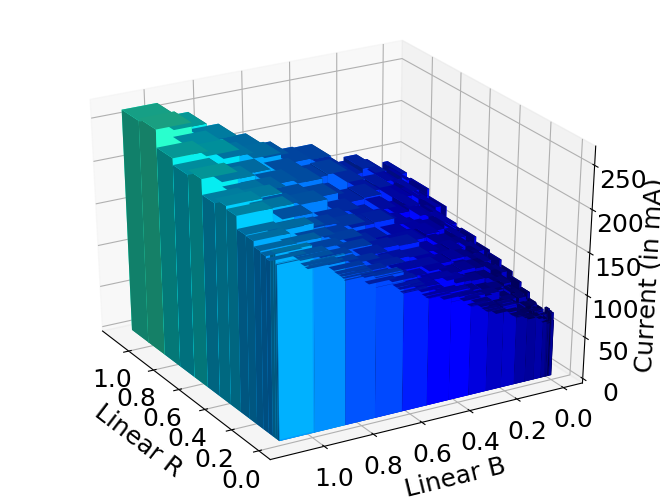
\includegraphics[width=\textwidth]{figure/002_Pixel2_monotonicity_cube.png}
		\caption{Pixel 2}
		\label{fig:initial_monotonicity_n6_w}
	\end{subfigure}
	\hfill
	\begin{subfigure}[]{0.28\textwidth}
		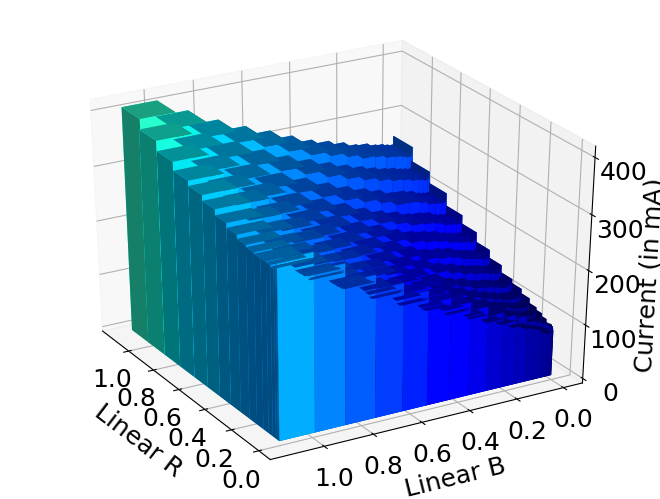
\includegraphics[width=\textwidth]{figure/003_MotoZ3_monotonicity_cube.png}
		\caption{Moto Z3}
		\label{fig:initial_monotonicity_p2_w}
	\end{subfigure}
	\hfill
	\begin{subfigure}[]{0.28\textwidth}
		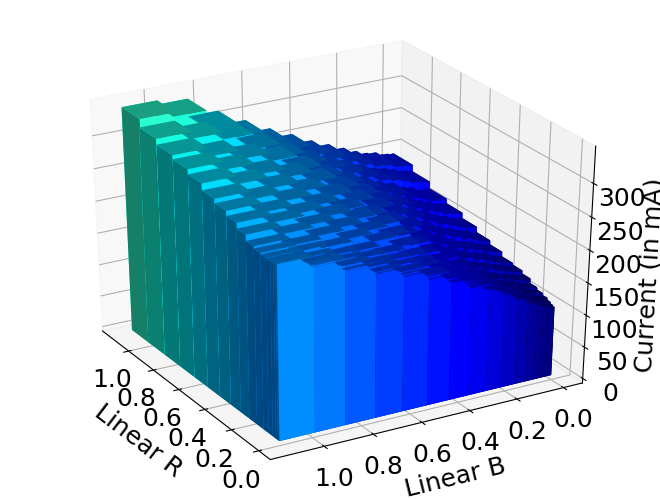
\includegraphics[width=\textwidth]{figure/004_Pixel4_monotonicity_cube.png}
		\caption{Pixel 4}
		\label{fig:initial_monotonicity_z3_w}
	\end{subfigure}
	\hfill
        \vspace{-0.1in}
	\caption{Measured pixel power values for a 2-D dissection of the 3-D color space on the three phones do not fall into a plane.}
\label{fig:initial_monotonicity}
\end{figure*}


\subsection{Key Insight}

Since the non-linear model (NLM) achieves similar accuracy as the linear model
with linear regression (LMLR), 
\comment{this needs to be confirmed by the numbers above???}
we discuss our key insight using the
LMLR model.
Recall that LMLR models the pixel power for any given RGB value
$(R_i, G_i,B_i)$ as a linear combination of the subpixel power 
$f(R_{i}), g(G_i)$, and $h(B_i$) (Eqn.~\ref{eq:linear_model_linear_regression}).
%  \begin{equation}
%  	P_i(R_i, G_i,B_i) = e_1\cdot f(R_{i}) + e_2\cdot g(G_{i}) + e_3\cdot h(B_{i}) + e_4
%  	\label{eq:linear_equation9}
%  \end{equation}
Since the subpixel power $f(R_{i}), g(G_i)$, and $h(B_i$) are linear
with respect to the subpixel linear RGB values
(Figure~\ref{fig:initial_evaluation_2}), their linear combination
should be able to and can only fit any plane in the 3-D coordinate space of
($Ri, G_i, B_i$). The question then becomes: do the pixel power values
$P_i(R_i, G_i,B_i)$ fall on a plane?
% in the 3-D color space?

Since it is hard to visualize the measured $P_i(R_i, G_i,B_i)$ in the
3-D RGB space, we select a dissection of the 3-D color space with a fixed
$G$ value (at 112), and plot the measured power value for the 2-D R-B space (in
linear RGB values) in Figures~\ref{fig:initial_monotonicity}(a)-(c) for
the three phones, where the height of the top surface shows the display power
draw values.  We see that the surface does not fall into a plane! This is
the key reason why any particular linear combination of subpixel power functions
(which are linear in the subpixel color) cannot approximate
the pixel power behavior well. In addition,
our experiments in \S\ref{subsec:nonlinear} showed
that adding non-linear terms cannot fit the nonlinear pixel power behavior well either.

We make a key observation that {\em although the pixel power values do not
fall in a plane across the entire color space, they correspond to a reasonably smooth surface,}
\eg as shown in the 2-D dissection example in Figure~\ref{fig:initial_monotonicity}. 
Therefore, if we cut the 3-D color space into small subgrids, the
pixel power values within each subgrid are likely to fit closely in
a flat plane and thus can be fitted well using linear combinations
of the subpixel (linear) power functions $f(R_{i}), g(G_i)$, and $h(B_i$).

Motivated by the above insight, we propose a new pixel power model
that can estimate the OLED display power with much better accuracy
than the prior art.  The basic idea of the new model is to divide the 3-D
color space (of dimension 256$\times$256$\times$256) into small subgrids
% (\eg of 16$\times$16$\times$16 sRGB values each)
and derive a piecewise LMLR model for each subgrid.

% \begin{equation}

% \begin{bmatrix}
%     y \\
%     m \\
%     c \\
%     w
% \end{bmatrix}
% =
% \begin{bmatrix}
%      0.544 &      1.489 &      0.000 \\
%      0.638 &      0.000 &      1.000 \\
%      0.000 &      1.193 &      0.739 \\
%     -0.201 &      4.125 &     -0.401
% \end{bmatrix}

% \end{equation}


\subsection{Model Derivation}
\label{subsec:modelderivation}

% Piecewise model (in RGB space)
% Linear (3 var vs. 4 var)
% Non-linear (8 var) <r+g+b+rg+bg+gr+rgb+c>
% precedural

Deriving the above piecewise pixel power model consists of three
steps: decomposition of the color space, data collection, and model
derivation for each sub color space.

\begin{figure}[tp]
	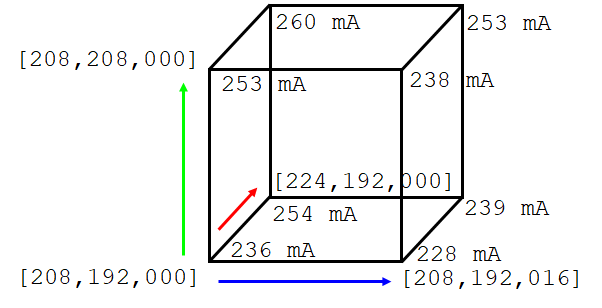
\includegraphics[width=0.35\textwidth]{./figure/004b_Cube_Model.png}
        \vspace{-0.1in}
	\caption{A 16$\times$16$\times$16 subgrid in the 3-D sRGB color space.}
        \vspace{-0.15in}
	\label{fig:cube_model}
\end{figure}
%   \begin{figure}[]
%   	\includegraphics[width=0.45\textwidth]{./figure/005_Cube_Zoom.png}
%   	\caption{How the cube in color space segmentation looks like.}
%   	\label{fig:cube_zoom}
%   \end{figure}


First, we decompose the 256$\times$256$\times$256 RGB color space into
subgrids of size $s\times$$s$$\times$$s$, where $s$ is the granularity of
the piecewise pixel power model. The choice of $s$ determines the
tradeoff between accuracy and the model size. The model size in turn
determines the memory and lookup
overheads. Figure~\ref{fig:cube_model} shows an example grid
of size 16$\times$16$\times$16 resulted from decomposing the
3-D color space into 16$\times$16$\times$16 subgrids.

Second, we experimentally measure the pixel power value as before
(\S\ref{subsec:super}) by displaying monochromatic images one at a time
corresponding to the color of each grid point in the decomposition. For
$16\times 16 \times 16$ subgrids, there will be $17^3 = 4913$ grid
points.

Finally, for each subgrid, we derive a pixel power model by applying linear regression 
to derive the coefficients of the model, \ie by fitting the power values at its 8 corner grid points
(see Figure~\ref{fig:cube_model}).  We
evaluate two model types for each subgrid, LMLR
(Eqn.~\ref{eq:first_order_variable}) and NLM (Eqn.~\ref{eq:second_order_variable}),
and denote the new models as P-LMLR (piecewise LMLR) and P-NLM (piecewise NLM):

\vspace{-0.1in}
{\small
  \begin{align}
	P^{grid_j}_i &= e_1^j\cdot f(R_i) + e_2^j\cdot g(G_i) + e_3^j\cdot h(B_i) + e_4^j
	\label{eq:first_order_variable} \\
  P^{grid_j}_i &= e_1^j\cdot f(R_i) + e_2^j\cdot g(G_i) + e_3^j\cdot h(B_i) + \label{eq:second_order_variable} \\
&  e_4^j\cdot f(R_i)g(G_i) +
  e_5^j\cdot f(R_i)h(B_i) +
  e_6^j\cdot g(G_i)h(B_i) +
  e_7^j \nonumber
\end{align}
}
\noindent
%The reason we add constants $e_4^j$ and $e_^j$ is because the power odes not start from

\vspace{-0.1in}
\paragraph{Handling color transformation.}
{For the cases with color transformations, \ie due to brightness level change,
%(on Pixel 2 and Moto Z3)
color mode change, or color correction,
 if  the color transformation, \ie the color matrix, is known,
 the new power model can be derived from the default power model;
 otherwise, the new power model needs to be experimentally generated.
}
% This is because the hardware composer changes the colors
% in hardware, which is in perceivable to the software.}

\if 0
Second major design aspect is to compute the OLED display current withing
16.7 ms. For this purpose we considered sampling of the image and found that
the relative error is small with sampling as seen in the
Figure\ref{fig:smaplinh_error}. The time taken for computation with various
sampling rates are shown in Figure\ref{fig:smapling_time} and we concluded
that even with sampling of less than 1\% we can get low relative error with
computation speed up. However to get the complete data for a full resolution
image it can take up to 2.5 seconds which is no where in our required limits
of 16.7 ms.
\fi

% \subsection{Model Design and Application}

% Model derivation
% training
% Using model online
% Memory-efficient sampling
% Table lookup the piecewise model
% Overhead evaluation

\if 0
\subsection{Model Training}

We created an android app which displays a mono-color image. This mono-colored
image corresponds to the edge of the cube explained above. R language was used
to generate the 4 variable linear equation to estimate power for each cube.

When deriving the power for the OLED display,we sampled 1\%  of the screen.
For each sampled pixel the matching color cube is selected and corresponding
equation is used to estimate the current consumed by the pixel. 
The current (power) is added up and extrapolated to obtain  the current for
the full screen.

We created an utility using OpenGL call to generate a virtual display.
The overhead to generate the virtual display is less than 5 ms per frame with a
power overhead of {TODO:power overhead J for Nexus 6, x J for
Moto Z3 and x J for Pixel 2.}
\fi



\subsection{Using Model in Real Time}
\label{subsec:appl}

Using the power model in real time includes four simple steps:
(1) Record a pixel frame, \eg via a vitual display,
% we can estimate its OLED power draw in three simple steps:
(2) For each pixel in the frame, find the sRGB subgrid it belongs to;
(3) Apply the piecewise pixel power model of that subgrid to
estimate the power draw for the pixel;
(4) Sum up the estimated power for all the pixels
(Eqn.~\ref{eq:linear_equation0}).

\dcomment {
On the same three phones,
once a frame is recorded in memory, Steps 2--4 only take
10ms, 10ms, and 4ms, respectively.  However, we found recording a single frame from
the virutal display can easily take hundreds of milliseconds, which
prevents the model from being used in real time, \eg by an
enhanced Android Battery (\S\ref{subsec:tool2})}

%  can incur significant computation overhead as modern
%  OLED displays come with millions of pixels.  {For example, the Nexus 6
%  OLED display has 8 million pixels, and calculating the power for
%  every pixel using the LMLR model in our highly optimized C
%  implementations takes 1 second on a Dell laptop.  }

\if 0
Pixel sampling was shown to effectively capture the distribution of
the pixel colors in a frame and reduce the cost of model application
for estimating the OLED power draw for a frame with a minimal impact
on accuracy~\cite{dong2009current}. The basic idea is to select a
subset of the pixels from the full frame, calculate their average
pixel power using the power model, and then extrapolate the average power to derive
the total power for the whole frame.
\fi

\dcomment{
To control the frame recording time to be a fraction of the 16.7ms
per-frame rendering time,
\if 0
we experimented with a few sampling strategies similarly as
in~\cite{dong2009current}, including random sampling which randomly
selects a fixed number of pixel and uniform sampling which selects
pixels with uniform spacing. We found that uniform sampling results in
similar accuracy as random sampling
but has slightly lower runtime overhead due to simpler
and more uniform memory access. We thus use uniform sampling in our
design.
\fi
we apply uniform pixel sampling (experimentally found to be faster than random sampling
yet give similar modeling accuracy) similarly as
in~\cite{dong2009current}.
We define {\em sampling ratio $K$} as the factor of reduction: one pixel is chosen from
the center of each grid of
$\sqrt{K}\times\sqrt{K}$ pixels.
The choice of the sampling ratio determines the tradeoff between
runtime reduction and modeling error.
We experimentally evaluate the tradeoff in the next section. NOT CORRECT. WAS RELEVANT IN NEXUS 6}

\dacomment{
On the same three phones,
% once a frame is recorded in memory,
Steps 1--4 takes
54ms, 58ms and 46ms, respectively.
This prevents the model from being used in real time, \eg by 
enhanced Android Battery (\S\ref{subsec:tool2}).
% \comment{
% However, we found recording \comment{and accessing} a single
% frame from the virtual display can easily take hundreds of milliseconds,
% which prevents the model from being used in real time, \eg by an
% enhanced Android Battery (\S\ref{subsec:tool2}).
% REMOVING THIS
% }
To control the Step 1--4 execution time
% frame recording time
to be within a fraction of the 16.7ms ,i.e,per-frame
rendering time, we apply uniform pixel sampling (experimentally found to
be faster than random sampling yet gives similar modeling accuracy) similar as to
described in~\cite{dong2009current}. We define {\em sampling ratio $K$} as the factor
of reduction: one pixel is chosen from the center of each grid of
$\sqrt{K}\times\sqrt{K}$ pixels. The choice of the sampling ratio determines
the tradeoff between runtime reduction and modeling error. We experimentally
evaluate the tradeoff in the next section. ADDED}

\if 0
\subsubsection{A user-level online tool}

An android app was created which can train itself for any phone which is equipped with an
OLED display. Once the OLED model is generated the app will give a real time display
power estimate on the screen. The current update of the power is kept at 1 sec but it can
be change to 60 time a second to match the 60 FPS display of the modern phone display.
\fi


%%%%%%%%%%%%%%%%%%%%%%%%%%%%%%%%%%%%%%%%%%%%%%%%%%%%%%%%%%%%%%%%%%%%%%%%%%%



\if 0
\subsection{Fast Modeling for Profiling a Single Frame}
\label{subsec:fast}

On newer phones such as Pixel 2 and Moto Z3, the built-in power sensor has a low
sampling rate, at approximately every 1.4 seconds. With this sampling rate,
the model generation process in \S\ref{subsec:modelderivation} will take approximately 12 hours for 4096
piecewise models and 1.4 hours for 512 piecewise models.
Though model generation is a one-time effort,
it can be too long for first-time use of the power model.
Furthermore, an app designer often has to test her app on various
devices before releasing the app, each requiring its own model generation.
%  So modeling and optimizing app in various devices is very time
%  consuming given that for a UI design consists of a small proportion of
%  colors.
We discuss a quick way of model generation, which can be used
in modeling the OLED power draw of a single frame on a new device.
%% \comment{factor of 8 dfference?}
%% This is because ???
%  This is because to ensure the experiment very
%  precisely during the long test duration, \ie the external
%  environmental conditions like temperature.

We observe that for the set of apps we experimented with (listed in
\S\ref{tab:experiments}), if we plot the histogram of the pixel colors
in the activity frames, a few distinct peaks (??to ???) account for a majority of
the frame pixels. This happens because the app activity UIs are
synthetically colored, and the app developer tends to use just a few colors
in the design. The remaining pixels have many colors spread in the
histogram with low frequencies which come from dynamic objects (\eg
images) in the frame which tend to have continuous textures.

%   the histogram is very distinct and has few peaks i.e. about 0.2\% of
%   the total number of images used to generate 16x16x16 model and 1.6 \%
%   of 32x32x32 model.  This shall take less than 2 minutes for the apps
%   as compared to hours for generate the complete model.


%  When designing the UI, the developer will not consider these
% objects as these are updated at the runtime.

Our fast model generation derives pixel power needed for modeling such
a typical frame as follows. First, we detect UI components in the frame to
identify dynamic components. We do this by using the Per-Frame OLED Power 
Analyzer (described in \S\ref{subsec:analyzer}).  Second, we generate the histogram
pixel colors to identify the peaks that correspond to the colors used
in the UI design. Third, we derive the pixel power draw for each of the few peak colors
following the methodology in \S\ref{sec:measurement},
each of which takes only 10 seconds. Finally,
we use the pre-generated simple LMLR model (dervied from four basic pixel colors)
to model the power draw of remaining pixels.
Though the LMLR model can be inaccurate, since it is only used for a small percentage of pixels,
\comment{what is the dynamic content is big???}
its error with respect to total display current will be very small.

\fi



\if 0
There might be some continuous components in the activity which may not contribute
to more than 1\% like the shadowing of the text. For this we switch to the linear model.
As we have seen earlier we estimate the red, blue and green curve in linear RGB,
by only knowing the lowest and highest intensity current. So in total for this we
require 4 (as the lowest intensity in all red, green and blue is black) images to evaluate the current.
The error in linear model is high but it will be a small fraction of the screen and
this error with respect to total display current will be very small.

We generate the histogram of the entire screen. We find all peaks which have
a contribution to the screen area more than 1\% of the screen area.
\fi

\if 0
\subsubsection{Implementation:}
We created an Android app for this purpose.
We brought the Android screencap command. We fetch
the screen and generate an histogram.
We identify the peaks. We go into a app training mode where the model is evaluated
by displaying monochromatic images on the screen. Each of the image is shown for 5 to 10
seconds.
If the peaks do not cover 99\% of the screen , we also calibrate 4 more images i.e.
black, read, green and blue at full intensity for linear model.
\fi



\subsection{Model Evaluation}
\label{sec:evaluation}

To evaluate the new model,
we implemented a power estimator consisting of
a sampling-based frame recorder
by modifying the Android screenrecord command code,
and a power calculator that implements Steps 2--4 in a C++ program with ~1 KLOC.
% using OpenCV Library.
It takes a pixel sampling ratio and the phone
display power model as input, records a frame,
and outputs the estimated display power consumption.
Below, we evaluate the accuracy and runtime of the
power estimator 
% running on the three phones
and how sampling affects their tradeoff.

% \subsection{Model Evaluation}

\if 0
We calculated the prediction error of the new model
in predicting the power at the center point of each color cube.
Using measured and estimated current, we calculated the error value.
The average error using linear and non-linear model was found to be less
than 5\%. For Nexus 6 , the average error is  3\% both both models. For Pixel 2,
average error was 2\% and 3\% for linear and non-linear model respectively.

We concluded from the above findings that linear model is good to use for
estimation,though non-linear model can provide us marginally better estimation.
This is because though the error is small in non linear model 
and the computation requirement in linear model is quite less in comparison
to non-linear model.
\fi


% \subsection{Accuracy}

\paragraph{Methodology.}
%  We evaluate the accuracy of the new pixel power model following the
%  same methodology as in \S\ref{sec:measurement}, \ie displaying static
%  images one at a time, recording the OLED display power reading from the
%  power sensor, and comparing the model estimated power against the
%  ground truth.
% We evaluate the accuracy of the new pixel power model with a set of 100
% images taken from Google Images, comprising both digitally generated and
% natural images. The set of images covers 10 diverse categories of content:
% Abstract, Animals, Birds and Fish,
% Cartoon, 3D CGI, Flower, Painting,
% Landscape, Plain, Fruits/Vegetables, and Mountains/Rivers.
% We evaluate the accuracy of the new pixel power model with a set of 100
% images taken from Google Images, comprising both digitally generated and
% natural images.
We evaluate the accuracy of the new pixel power model with a set of screenshots
 for 5 activities each for 6 popular Google apps,
Calculator, Calendar, Maps, Phone, News, and YouTube,
under both dark and light modes.
We measure the ground truth OLED power
following the same methodology as in \S\ref{sec:measurement}.
\forjnl{as shown in Figure~\ref{fig:100_images_expriment}.}
% including Abstract, Animals, Birds \& Fish, Cartoon, 3D CGI, Flower,
% Painting, Landscape, Plain, Fruits \& Vegetables, and Mountains \& Rivers.
To evaluate the impact of pixel sampling, we vary the sampling ratio
from 1 (no sampling) to 4096.
% The runtime of model application was measured on a Windows laptop.

% We want to evaluate the OLED current model with running our app. The limitation being
% that there can be various other current consuming components in the mobile phone
% like CPU, GPU to state a few and these are also required to be accurately
% modelled to extract a very accurate OLED screen power. We considered a middle path
% and decided to use an Android app ExoPlayer which has a very low overhead , so that
% we can extract the OLED display current more accurately.


\paragraph{Impact of subgrid size.}
We first measure the prediction error of P-LMLR and P-NLM models across
% the 100 images
the activity screenshots from the 6 Google apps
under subgrid sizes 16 and 32, on the three phones, respectively.
The results show that using subgrid sizes 16 and 32 result in very similar
prediction errors.  Since using subgrid size
16 only needs 64KB 
to store the 4096 piecewise models (of 4 coefficients each),
which is insignificant, and incurs
negligible application time (see below),
but can better cope with potential OLED power fluctuations (\eg on other phones),
% from being able to fit the piecewise models
% in the L2 cache when processing on a laptop.
we use subgrid size $16\times 16\times 16$ in our model design.

\if 0
\begin{figure*}[th]
	\begin{subfigure}[]{0.29\textwidth}
		\includegraphics[width=\textwidth]{./figure/700_100Image_N6_Standard.pdf}
		\caption{Nexus 6}
	\end{subfigure}
	\hfill
	\begin{subfigure}[]{0.29\textwidth}
		\includegraphics[width=\textwidth]{./figure/703_100Image_P2_Boosted.pdf}
		\caption{Pixel 2}
	\end{subfigure}
	\hfill
	\begin{subfigure}[]{0.29\textwidth}
		\includegraphics[width=\textwidth]{./figure/701_100Image_Z3_Vibrant.pdf}
		\caption{Moto Z3}
	\end{subfigure}
        \vspace{-0.1in}
	\caption{Measured and predicted OLED power draw using P-LMLR
          for 100 images in 10 categories (A: Abstract, B: Animals, Birds and Fish,
			C: Cartoon, D: 3D CGI, E: Flower, F: Painting, G: Landscape, H: Plain,
			I: Fruits / Vegetables, J: Mountains / Rivers).}
	\label{fig:100_images_expriment}
\end{figure*}
\fi


\paragraph{Impact of sampling ratio.}
Figure~\ref{fig:smapling_error} left shows the additional
prediction error of P-LMLR when increasing the pixel sampling ratio
compared to that of P-LMLR without sampling,
for the set of activity screenshots from the 6 Google apps on the 3 phones.
% The error here is calculated w.r.t. to the current estimated with no sampling as base value.
We see that increasing the sampling ratio increases the prediction error
slowly. The additional error predicted is less than 1\% for the
3 phones at the sampling ratio of 100.

% \begin{figure}[tp]
% 	\begin{subfigure}[]{\columnwidth}
% 		\includegraphics[width=0.48\columnwidth]{./figure/501_N6_error.pdf}
%  		\includegraphics[width=0.48\columnwidth]{./figure/502_N6_time.pdf}
% 		\caption{Nexus 6}
% 	\end{subfigure}
% 	
% 	\begin{subfigure}[]{\columnwidth}
% 		\includegraphics[width=0.48\columnwidth]{./figure/503_P2_error.pdf}
%  		\includegraphics[width=0.48\columnwidth]{./figure/504_P2_time.pdf}
% 		\caption{Pixel 2}
% 	\end{subfigure}
% 	\begin{subfigure}[]{\columnwidth}
% 		\includegraphics[width=0.48\columnwidth]{./figure/505_Z3_error.pdf}
%  		\includegraphics[width=0.48\columnwidth]{./figure/506_Z3_time.pdf}
% 		\caption{Moto Z3}
% 	\end{subfigure}
%         \vspace{-0.1in}
% 	\caption{Prediction error of and runtime in applying the P-LMLR model under various
%           sampling ratios.}
%        \vspace{-0.1in}
% 	\label{fig:smapling_error}
%        \vspace{-0.1in}
% \end{figure}

% \begin{figure}[tp]
% 	\begin{subfigure}[]{\columnwidth}
% 		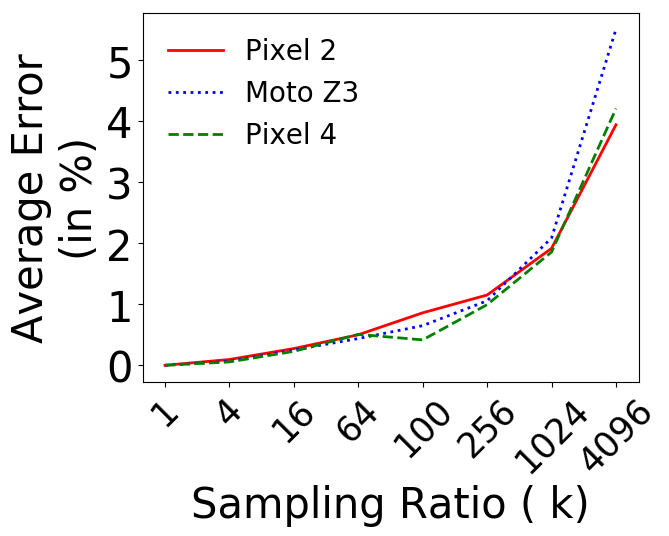
\includegraphics[width=0.48\columnwidth]{figure/001_sampling_ratio_error.png}
%  		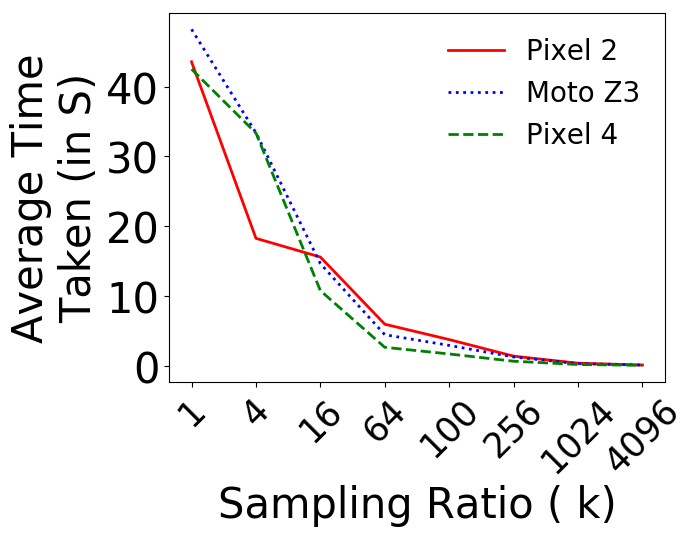
\includegraphics[width=0.48\columnwidth]{figure/002_sampling_ratio_time.png}
% 	\end{subfigure}
%         \vspace{-0.1in}
% 	\caption{Prediction error of and runtime in applying the P-LMLR model under various
%           sampling ratios.}
%       \vspace{-0.1in}
% 	\label{fig:smapling_error}
%     %\vspace{-0.1in}
% \end{figure}

\begin{figure}[tp]
	\begin{subfigure}[]{0.48\columnwidth}
		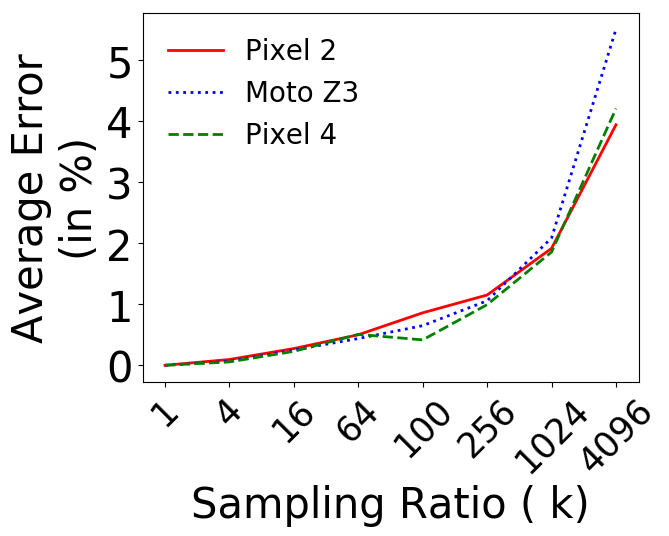
\includegraphics[width=\columnwidth]{figure/001_sampling_ratio_error.png}
		\caption{Additional model error}
		\label{fig:eval_smapling_error_error}
	\end{subfigure}
	\begin{subfigure}[]{0.48\columnwidth}
 		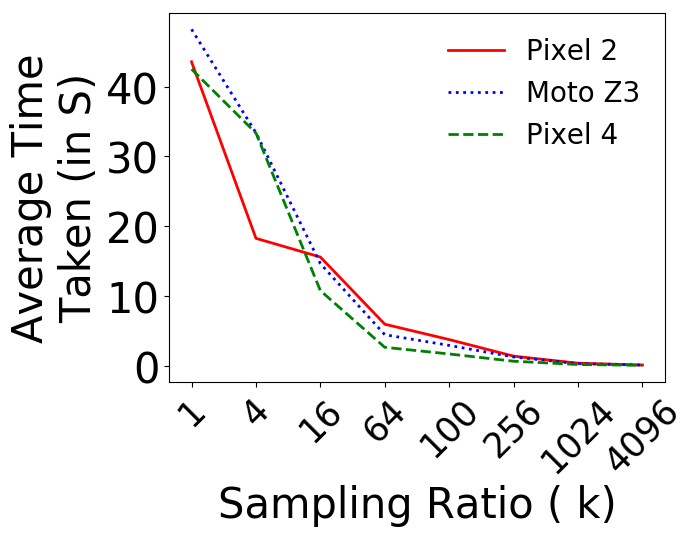
\includegraphics[width=\columnwidth]{figure/002_sampling_ratio_time.png}
 		\caption{Average runtime (T1+T2)}
 		\label{fig:eval_smapling_error_time}
	\end{subfigure}
	\vspace{-0.1in}
	\caption{Additional prediction error of and runtime in applying the P-LMLR model under various
          sampling ratios.}
	\label{fig:smapling_error}
    \vspace{-0.1in}
\end{figure}

%% This for the phone results. Above is the computer results
% \begin{figure}[tp]
% 	\begin{subfigure}[]{\columnwidth}
% 		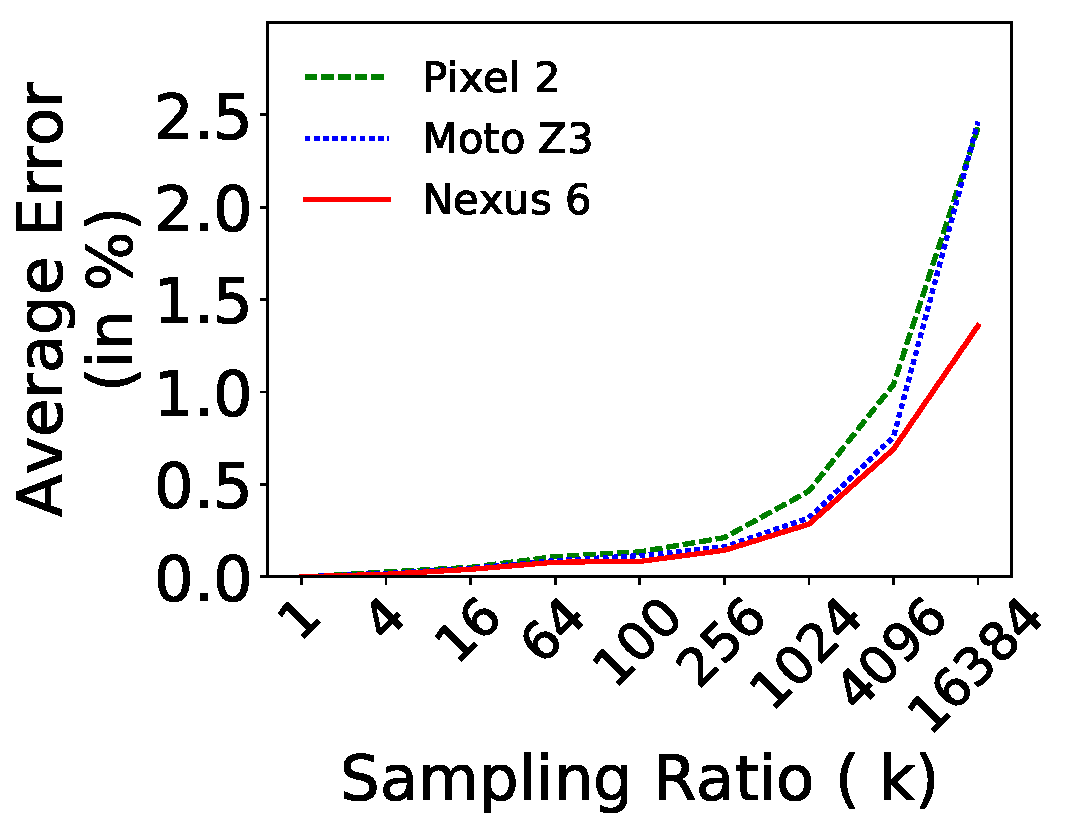
\includegraphics[width=0.48\columnwidth]{./figure/511_All_error.pdf}
%  		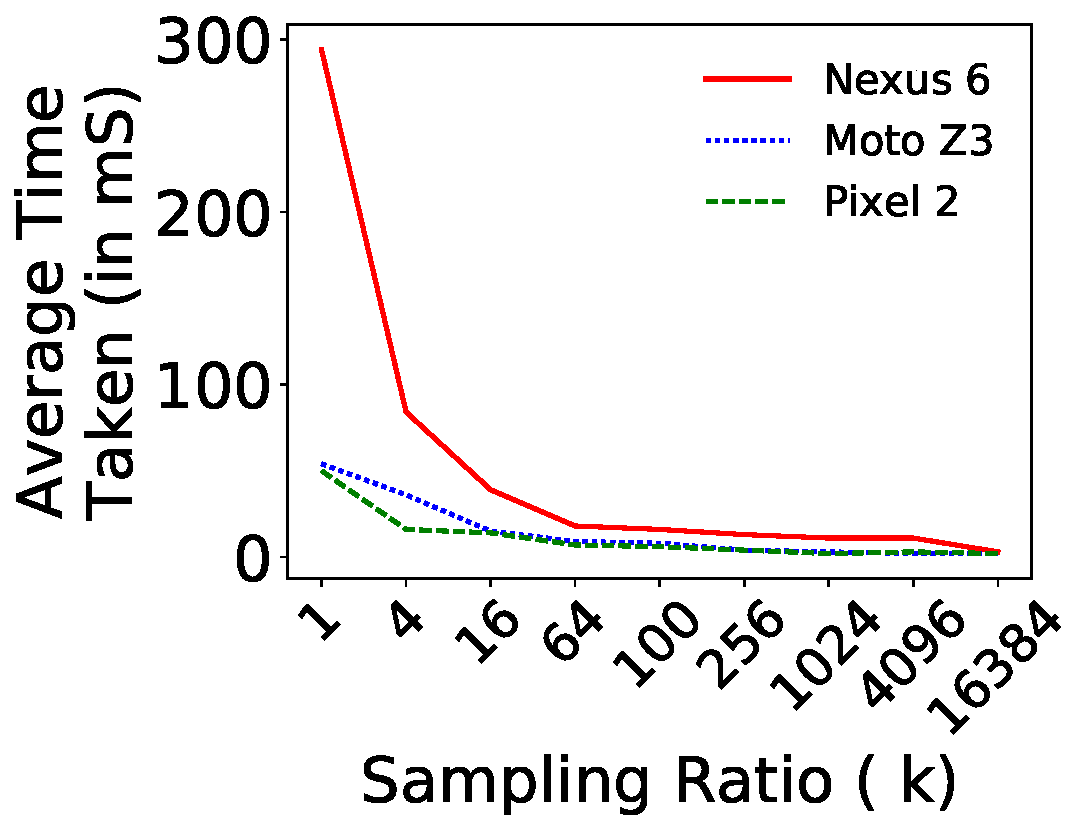
\includegraphics[width=0.48\columnwidth]{./figure/511b_All_time.pdf}
% 	\end{subfigure}
%         \vspace{-0.1in}
% 	\caption{Prediction error of and runtime in applying the P-LMLR model under various
%           sampling ratios.}
%        \vspace{-0.1in}
% 	\label{fig:smapling_error}
%        \vspace{-0.1in}
% \end{figure}

% \subsection{Model Application Runtime}

%  \paragraph{Methodology}
%  Further our Power model c++ program also generate the runtime overhead
%  incurred at various sampling ratios for the 100 images. 
%  As mentioned earlier, we used the sampling ratio from 0.01 \% to 90 \% and
%  %  ran this experiments on the server and during this we measured run time over heads. \dcomment{Get Specs}

\paragraph{Frame recording and power calculation time.}
Figure~\ref{fig:smapling_error} right shows how the sampling
ratio affects the total time (frame recording time (T1) 
plus power calculation
time (T2)) in applying the P-LMLR model to
calculate the power for a given frame.
%   {
%   This contains the frame capture and model application overhead.
%   Without sampling, the computation takes 8.3 ms, 4.4 ms and 4.1 ms on
%   the 3 phones which less than 10\% on the total time taken.
%   }
We observe that for all three
phones, the total time and two individual times not shown are inversely proportional to the
sampling ratio. In particular, without sampling, the frame recording
time are 10ms, 10ms, and 4ms
and
the power calculation time are 44ms, 48ms and 42ms on
 the three phones,
while with a sampling ratio of 100, the recording time are reduced to
1ms, 1ms, and 1ms, and power calculation time are reduced to
4ms, 3ms, and 2ms, respectively.
We note the long frame recording time is due to the delay in pulling data from frame buffer
and does not keep CPU busy.
As we will show in \S\ref{subsec:tool2},
the average CPU utilization of power calculation
is only 1.1\%, 0.9\%, and 0.6\% on Pixel 2, Moto Z3, and Pixel 4, respectively.
\if 0
The reduced model application runtime allows the OLED display power to
be calculated for a recorded app run (one frame every 16.7ms at 60
FPS) at less than 1/10th of the app run duration, in
post-processing.
\fi
We thus conclude that a sampling ratio of 100 strikes
a good balance between minimal prediction accuracy loss and sufficient
model application runtime reduction.

% \begin{figure}[]
% 	\includegraphics[width=\columnwidth]{./figure/401_Model_Compariosn.png}
% 	\caption{The heat map of the display current shows the different in the OLED
% 		model between the two generatios of the OLED display technology}
% 	\label{fig:oled_model_comparison}
% \end{figure}

% \begin{figure*}[tp]
% 	\begin{subfigure}[]{0.33\textwidth}
% 		\includegraphics[width=\textwidth]{./figure/200_n6_simple.pdf}
% 		\caption{Nexus 6}
% 	\end{subfigure}
% 	\begin{subfigure}[]{0.33\textwidth}
% 		\includegraphics[width=\textwidth]{./figure/201_z3_vibrant.pdf}
% 		\caption{Moto Z3 Neutral Standard Color Mode}
% 	\end{subfigure}
% 	\begin{subfigure}[]{0.33\textwidth}
% 		\includegraphics[width=\textwidth]{./figure/201_z3_vibrant.pdf}
% 		\caption{Moto Z3 Neutral Vibrant Color Mode}
% 	\end{subfigure}
% 	\hfill
% 
% 	\centering
% 	\begin{subfigure}[]{0.33\textwidth}
% 		\includegraphics[width=\textwidth]{./figure/203_p2_boosted.pdf}
% 		\caption{Pixel 2 Boosted Color Mode}
% 	\end{subfigure}
% 	\begin{subfigure}[]{0.33\textwidth}
% 		\includegraphics[width=\textwidth]{./figure/204_p2_natural.pdf}
% 		\caption{Pixel 2 Natural Color Mode}
% 	\end{subfigure}
% 	\begin{subfigure}[]{0.33\textwidth}
% 		\includegraphics[width=\textwidth]{./figure/205_p2_staturated.pdf}
% 		\caption{Pixel 2 Saturated Color Mode}
% 	\end{subfigure}
% 
% 	\caption{The current consumed by the OLED display with varying RGB values
%         on three phones, Nexus 6, Moto Z3 Plus (2 color modes), and Pixel 2 (3 color modes).}
% 	\label{fig:initial_evaluation}
% \end{figure*}

% \begin{figure}[!htb]
% 	\centering
% 	\begin{tabular}[t]{|c|c|}
% 	\hline
% 	
%     \begin{subfigure}{0.4\textwidth}
%     \centering
%     \smallskip
%     \includegraphics[width=0.9\linewidth,height=1.7\textwidth]{./figure/904_Current_Model_Comparision.png}
%     \caption{Cat 1} %{Light Unit}
% \end{subfigure}
%     &
%         \begin{tabular}{c}% if you add [t], than sub images are pushed down
%         \smallskip
%             \begin{subfigure}[t]{0.4\textwidth}
%                 \centering
%                 \includegraphics[width=0.9\textwidth]{./figure/900_BASE_Model_Comparision.png}
%                 \caption{Cat 2}
%             \end{subfigure}\\
%             \begin{subfigure}[t]{0.4\textwidth}
%                 \centering
%                 \includegraphics[width=0.9\textwidth]{./figure/903_P2_Model_Comparision.png}
%                 \caption{Cat 3}
%             \end{subfigure}
%         \end{tabular}\\
% \hline
%     \end{tabular}
%     \caption{Cats}
% \end{figure}

% \begin{table}[h]
% \begin{center}
% 	\centering
% 	\caption{Popular Google Android App Experiment Methodology}
% 	\begin{tabular*}{\columnwidth}{@{\extracolsep{\fill}}| l | l | r |}
% 		\hline
% 		Phone        & Average Error & Average Time\\
% 		\hline
% 		Nexus 6      & .06 \%        & 11 \\
% 		Moto Z3      &  2.9 \%        & 11 \\
% 		Pixel 2      & 	1.7 \%        & 11 \\
% 		\hline
% 	\end{tabular*}
% 	\label{tab:100_images}
% \end{center}
% \end{table}


% \begin{table}[tp]
% \begin{center}
% \centering
% \caption{Mean (median) display power prediction error for the 6 app activity screenshots.}
% %  (50 percentile | 90 percentile)
% % \dcomment{Showing both numbers. Not to be included in final}
% \vspace{-0.1in}
% \footnotesize
% % \begin{tabular*}{\columnwidth}{ | p{0.12\columnwidth} | p{0.20\columnwidth} | p{0.20\columnwidth} | p{0.20\columnwidth} | p{0.20\columnwidth}  }
% \begin{tabular*}{\columnwidth}{@{\extracolsep{\fill}}|p{10mm}|c|c|c|c|c|}
% 	\hline
% 	       \multirow{2}{*}{Phone} & \multirow{2}{*}{Mode} & \multicolumn{4}{c|}{Average Percentage Error} \\
% 	\cline{3-6}
% 	        &   & LMLR & NLM & P-LMLR & P-NLM\\
% 	\hline
% 	{Pixel } & dark   & 21.6 ( 23.3) & 12.8 ( 13.5) & 4.2 ( 3.9) & 3.5 ( 2.3) \\
% 	                         % \cline{2-6}
% 	       2                  & light  & 7.2 ( 7.5) & 5.4 ( 5.5) & 1.7 ( 1.5) & 1.7 ( 1.5) \\
% 	\hline
% 	{Moto } & dark   & 17.3 ( 20.1) & 11.8 ( 13.7) & 3.1 ( 3.1) & 3.5 ( 3.6) \\
% 	                         % \cline{2-6}
% Z3	                         & light  & 5.0 ( 5.6) & 4.8 ( 5.5) & 2.2 ( 2.0) & 2.3 ( 2.1) \\
% 	\hline
%     {Pixel } & dark   & 18.9 ( 17.0) & 13.1 ( 11.8) & 4.3 ( 4.5) & 4.6 ( 4.6) \\
%                              % \cline{2-6}
%           4                  & light  & 6.5 ( 7.4) & 7.5 ( 7.9) & 2.6 ( 1.0) & 2.7 ( 0.9) \\
% 	\hline
% \end{tabular*}
% \label{tab:100_images}
% \end{center}
% \vspace{-0.15in}
% \end{table}

\begin{table}[tp]
\begin{center}
\centering
\caption{Mean (median) display power prediction error for the 6 app activity screenshots.}
\vspace{-0.1in}
{ \footnotesize
    \begin{tabular}{|p{7mm}|p{6mm}|c|c|c|c|}
    	\hline
    	       \multirow{2}{*}{Phone} & \multirow{2}{*}{Mode} & \multicolumn{4}{c|}{Average Percentage Error} \\
    	\cline{3-6}
    	        &   & LMLR & NLM & P-LMLR & P-NLM\\
    	\hline
    	Pixel & dark   & 21.6 (23.3) & 12.8 (13.5) & 4.2 (3.9) & 3.5 (2.3) \\ % \cline{2-6}
    	    2 & light  & 7.2 (7.5) & 5.4 (5.5) & 1.7 (1.5) & 1.7 (1.5) \\
    	\hline
    	Moto  & dark   & 18.9 (17.0) & 13.1 (11.8) & 4.3 (4.5) & 4.6 (4.6) \\ % \cline{2-6}
           Z3 & light  & 6.5 (7.4) & 7.5 (7.9) & 2.6 (1.0) & 2.7 (0.9) \\
    	\hline
        Pixel & dark   & 17.3 (20.1) & 11.8 (13.7) & 3.1 (3.1) & 3.5 (3.6) \\ % \cline{2-6}
            4 & light  & 5.0 (5.6) & 4.8 (5.5) & 2.2 (2.0) & 2.3 (2.1) \\
    	\hline
    \end{tabular}
}
\label{tab:100_images}
\end{center}
\vspace{-0.2in}
\end{table}
% \footnotetext{The error depends on the images tested as it is content specific.}

\paragraph{Accuracy.}
\forjnl{Figure~\ref{fig:100_images_expriment} shows the measured and predicted
OLED power draw using the new piecewise linear model (P-LMLR) for the
100 images and the prediction error for each on the three phones. We
see that using P-LMLR, the estimated OLED display power closely follows
the measured power for all 3 phones.}
Table~\ref{tab:100_images}
summarizes the average prediction error by LMR, NLM, P-LMLR, and P-NLM
for the activity screenshots with 100x sampling on the three phones.
The error for LMLR and NLM varies across the phones,
because their error for individual pixel colors vary in different regions of the color space
on different phones (Figure~\ref{fig:initial_evaluation_2})
and different images have different distribution of pixel colors.
In contrast, the prediction errors of P-NLM and P-LMLR are
almost identical and consistent across the 3 phones,
\ie the two models are robust to phone diversities,
% (within 10\%),
and the errors are significantly lower than that of LMLR and NLM.
In particular, P-LMLR reduces the average prediction error
of LMLR by
    5.1$\times$, 5.5$\times$ and 4.4$\times$ for dark mode
    and 4.2$\times$, 2.3$\times$ and 2.5$\times$ for light mode for the three phones.
%     \nexuserrorreduction,
%     \pixelerrorreduction, and
%     \motoerrorreduction,
%     from
%     \nexuserror, \pixelerror, and \motoerror
% down to 3.3\%, 3.3\%, and 2.9\% on the 3 phones.

% \dcomment{Add this}
% We recorded the screen from various apps and play it on the Android app and
% compared to the ground truth. We used a CPU and GPU model \dcomment{cite}
% to find the accuracy of the OLED model to be .


\section{OLED Power Profiling Tools}
\label{sec:tools}

Using the new OLED power model presented in \S\ref{sec:newmodel}, we
have developed two OLED power profiling tools.
%  and an Enhanced Android Battery which provides much more accurate OLED
% power and energy draw estimation than the default Android Battery.

\subsection{Tool 1: Per-Frame OLED Power Profiler}
\label{subsec:analyzer}


% The first tool, a per-frame OLED power  (PFOP) profiler,
\name is a per-frame OLED power profiler designed to enable
an app developer to profile and optimize the OLED power draw of all the
UI components known as views in Android in each app activity design.
The objects in these views fall into two broad categories:
dynamic objects and static objects. Since dynamic objects such as ads or videos
will change in real time, the developer typically focuses on
optimizing the power draw of static objects.
A second design goal of \name is to make it easy-to-use and portable
to any unmodified Android versions.
%  The PFOP analyzr assist the developer to rapidly analyse their apps for
%  display power optimization.

%   Further various views of an App might be designed at different timelines and by different
%   groups. The knowledge of views which are required to be optimized also increases the group
%   productivity, focusing direct effort on these least optimized parts.

%   We observed that Pixel2 and MotoZ3 has a power sensor with
%   sampling rate of approximately 1.4 second. Using this sampling
%   rate the static model generation will take more 12 hrs with 4096
%   piecewise model and more than 1.4 hrs with 512 piecewise model.
%   The main problem here is that we have to take care of the
%   experiment very precisely during the long test duration, i.e. the
%   external environmental conditions like temperature.


%    This happens because the activities are synthetically colored
%    and spread in the histogram happens in case there is a
%    dynamic object which may have continuous textures. When designing
%    the UI, the developer will not consider these objects as these are updated
%    at the runtime.

%   This is also true that designer has to evaluate their app on various devices
%   before they release the app. So modeling and optimising app in various devices is very time
%   consuming and given that UI design consists of a small proportion of colors.

The main challenge of the \name profiler design is to identify all the UI
components of the displayed frame, \eg separating dynamic objects from
static objects, in order to calculate their corresponding OLED power
draw.
% 
% The Challenge is to analyse and determine content of views. Our analysis 
%  determines what are the types of object present on the screen.For example
%  an ImageView or VideoView can be used to determine the dynamic objects.
%  Once the dynamic objects are identified we get it's bounding boxes.
We also need to remove system components on the screen such as the
status bar and the navigational bar.
%  which may also be static.
%   Once all the above mentioned components are removed, the remaining are
%   of the static objects which are for the activity of our interest
%   needing optimisation.


\if 0
There might be some continuous components in the activity which may not contribute
to more than 1\% like the shadowing of the text. For this we switch to the linear model.
As we have seen earlier we estimate the red, blue and green curves in linear RGB,
by only knowing the lowest and highest intensity current. So in total for this we
require 4 more, i.e. red, blue \& green at highest intensity and black
(as for the lowest intensity in all red, green and blue is black) images to evaluate the current.
The error in linear model is high but as it will be a small fraction of the screen,
this error with respect to total display current will be very small.
\fi

\if 0
We generated the histogram of the entire screen. We find all peaks
which have a contribution to more than 1\% of the screen area.  We use
this peaks to generate monochromatic images and generate the current
model for these specific images.  If the peaks doesn't cover 96\% of
the screen we capture an extra of 4 more images (black, red, green and
blue) in the linear model for the remaining of the screen.
\fi

%   For the per component analysis, the most straight forward way is to get
%   the view group of the entire screen and found that this information is
%   not readily available from the system.

The \name profiler breaks down the OLED power draw by a frame in three steps.
First, to identify all the UI
components in a frame, it uses the Android tool ``uiautomator'' to
obtain a dump of the current app screen in xml. {Analyzing the xml
  file gives information about the various views including all the
  system components on the app screen and their bounding boxes.}
Because the system UI components are outside the app view hierarchy,
\name uses the Android command ``dumpsys window windows'' to gather their
bounding boxes.  Second, \name uses the OpenCV library to extract the
pixels within each bounding box.  Finally, it applies the P-LMLR pixel
power model (Eqn.~\ref{eq:first_order_variable}) to derive the OLED power draw for each bounding box and
hence the UI component.


% \paragraph{Implementing the tool as an app.}
To make it easy to use and portable (second design goal),
we implemented the \name profiler as an Android
app that only
%   Since an app cannot directly call ``uiautomator'', we created a
%   background running process which calls ``screencap'' to capture
%   the screen shots.  Building the tool
uses built-in tools uiautomator,
dumpsys and screencap.
%   which makes it portable to Android devices with different (unmodified) Android OS versions.
%   In future work, we plan to implement
%   these as system binder \comment{does this require modiying android???}
%   for even lower overhead via piggybacking
%   surface flinger.
\begin{figure}[tp]
	\begin{subfigure}[]{0.30\columnwidth}
		\includegraphics[width=\textwidth]{figure/001_app_capture.png}
		\caption{Floating icon}
		\label{fig:tool1_screenshot_a}
	\end{subfigure}
        \hfill 
%%	\begin{subfigure}[]{0.40\columnwidth}
%%		\includegraphics[width=\textwidth]{./figure/12000b_model.png}
%%		\caption{Show Histogram and option of model}
%%		\label{fig:tool1_screenshot_b}
%%	\end{subfigure}
%%      \\
	\begin{subfigure}[]{0.30\columnwidth}
		\includegraphics[width=\textwidth]{figure/003_app_histogram.png}
		\caption{Histogram of pixel colors}
		\label{fig:tool1_screenshot_d}
	\end{subfigure}
        \hfill 
	\begin{subfigure}[]{0.30\columnwidth}
		\includegraphics[width=\textwidth]{figure/002_app_break_down.png}
		\caption{Per-UI component current}
		\label{fig:tool1_screenshot_c}
	\end{subfigure}
        \vspace{-0.1in}
	\caption{The \name profiler screen shots on Pixel 4.}
	\label{fig:tool1_screenshot}
    \vspace{-0.2in}
\end{figure}
Figure~\ref{fig:tool1_screenshot} shows the screen shots of the
profiler app in action. The app displays a floating icon which is an Android service
that overlays on top of the app that is running, as shown
in Figure~\ref{fig:tool1_screenshot_a}. Whenever the icon is pressed, it sends
a message to the background process to capture the screen and screen
layout via uiautomator.
\forjnl{The app then prompts a model selection
  activity where the developer can select fast model or pre-generated static model.
  }
% Figure~\ref{fig:tool1_screenshot_b}.  Analysis is shown as
% histogram which shows the color peaks and the time for generating the fast model.
%  The user is given a choice whether to choose fast model or
% the static model.
%   If fast model is selected,
%   the model generation
%   is started, and the user do not have to interact during model
%   generation. Analysis of the Fast model is shown as
For screen analysis, the app can toggle between two outputs.
%  component bounding
% box drawn and the histogram as shown in Figure~\ref{fig:tool1_screenshot_d}.
The first is a histogram showing the number of color peaks in the frame,
% and the time required for fast model generation,
as shown in Figure~\ref{fig:tool1_screenshot_d}.
%   If static model is chosen, is got from the app data.
% Once the model is chosen,
The second is the bounding box of
each selected view and the current per view at 100\%
brightness, as well as the total screen current at 30\%, 50\% and 100\%
brightness, as shown in Figure~\ref{fig:tool1_screenshot_c}.
%  We can chose the components to analyse by selecting the check boxes against them.
%   The app can save the selection,
%   \ie components bounding box and the full screen histogram.
%   We use this tool for our case study.

% We brought the Android screenrecorder and screencap command code. We fetch
% the screen and generate an histogram.
% We identify the peaks. We go into a app training mode where the model is evaluated
% by displaying monochromatic images on the screen. Each of the image is shown for 5 to 10
% seconds.
% If the peaks do not cover 99\% of the screen , we also calibrate 4 more images i.e.
% black, read, green and blue at full intensity for linear model.
% 
% We take the xml file generated by uiautomator to process and generate the bounding boxes
% for every view component.We also identify the type of the views.
% 
% The above display analyser tool is packaged into an android app for ease of use.App provides 
% a per components list for display as output at the end of the analysis.

\begin{table}[tp]
\begin{center}
	\centering
	\caption{\name profiler runtime breakdown (in seconds).}
	\label{tab:tooloverhead}
        \vspace{-0.1in}
    {\footnotesize
                \begin{tabular*}{\columnwidth}{ | p{0.45\columnwidth} | p{0.12\columnwidth} | p{0.12\columnwidth} | p{0.12\columnwidth} | }
  	% \begin{tabular*}{\columnwidth}{|l|c|c|c|}
		\hline
		Tool component        	&  Pixel 2 & Moto Z3 & Pixel 4\\
		\hline
		Screen shot	        	&  0.41 & 0.58 & 0.42 \\
		Gathering Bounding box  &  0.38 & 1.08 & 1.84 \\
		Per-UI component current	&  1.47 & 1.32 & 1.84 \\
		Generating Histogram	&  0.14 & 0.15 & 0.17 \\  
		Total frame current     &  0.02 & 0.02 & 0.03 \\
		\hline
	\end{tabular*}
	}
\end{center}
\vspace{-0.15in}
\end{table}

\paragraph{Evaluation.}
Since \name is an offline profiler,
we analyze the time it takes to analyze the OLED power draw of a frame.
We break down the time due
to its 5 processing steps: taking a screen shot, gathering the bounding box
data, generating per-UI component current, screen histogram generation,
and calculating the total current for the screen.  The results for the
three phones are shown in Table~\ref{tab:tooloverhead}.  We see that
taking screen shot, gathering bounding boxes, and histogram generation can
take a few seconds. This is the price we pay
for designing \name to be portable, \ie  only using system
commands on unmodified Android phones which do not use sampling.
Nonetheless, the total time for analyzing a frame is less than 4.3
seconds on all three phones.



\if 0
On average the screen shot took for 1.77s for Nexus 6, 617
ms for Pixel 2 and 547ms for Moto Z3.  For gathering bounding box
information, it took on average for 2.56 S for Nexus 6, 1.69 S for
Pixel 2 and 1.54 S for Moto Z3.  The total screen current computation
on an average took 395 mS for Nexus 6, 43 mS for Pixel 2 and 51 mS for
Moto Z3.  Per component current computation depends on the complexity
of the activity. On an average it took for 320 mS for Nexus 6, 132 mS
for Pixel 2 and 147 mS for Moto Z3.  The histogram generation took on
average 3939 mS for Nexus 6, 602 mS for Pixel 2 and 786 mS for Moto
Z3.  After the initial computation the data is stored in memory so
that the toggling between the components selection has very low
overhead.
\fi

\forjnl{Fast modeling depends on the number of peaks in the histogram which
greatly depends on the contents of the screen. On average we observed
that for the chosen app in Table~\ref{tab:activities_peaks} it took
less than 2 minutes on average (8 peak colors for the frame and 4 basic colors
for training the LMLR model).
}

% The screen shot of the output of the app is given in Figure~\ref{fig:tool2_screenshot}.
% \begin{figure}[]
% 	\begin{subfigure}[]{0.4\columnwidth}
% 		\includegraphics[width=\textwidth]{./figure/12000a_per_component_bounding_box.png}
% 		\caption{The app detects the bounding boxes as red of the views.}
% 	\end{subfigure}
% 	\begin{subfigure}[]{0.4\columnwidth}
% 		\includegraphics[width=\textwidth]{./figure/12000b_per_component_list.png}
% 		\caption{The app lists all the per component power.}
% 	\end{subfigure}
%         \vspace{-0.1in}
% 	\caption{Tool 1: Per Component Analyser. \dcomment{Not Complete Yet}}
% 	\label{fig:tool1_screenshot}
% \end{figure}

\if 0
\begin{table}[th]
\begin{center}
	\centering
	\caption{Average number of peaks over activities studied in the popular Google Apps.
		(0.2\% of ratio of 16x16x16 color cube takes 40 to 120 seconds depending of the
		 sampling rate.)}
	\label{tab:activities_peaks}
        \vspace{-0.1in}
	% \begin{tabular*}{\columnwidth}{@{\extracolsep{\fill}}| l | l |}
	\small {
	\begin{tabular*}{\columnwidth}{ | p{0.25\columnwidth} | p{0.14\columnwidth} | p{0.14\columnwidth} | p{0.3\columnwidth} | }
		\hline
		App Name        	&  Dark Mode & Light Mode & Ratio compared to 16x16x16 color cube\\
		\hline
		Calculator		&  3.7 & 3.3 & 0.09 \%\\
		Phone			&  3.1 & 2.5 & 0.08 \%\\
		Google Calender		&  3.6 & 3.5 & 0.09 \%\\
		Google Maps		&  8.3 & 7.8 & 0.20 \%\\  
		News			&  4.7 & 3.3 & 0.11 \%\\
		YouTube			&  6.2 & 5.6 & 0.15 \%\\
		\hline
	\end{tabular*}
	}
\end{center}
\vspace{-0.15in}
\end{table}
\fi
% To evaluate the accuracy of the app we choose various activities listed in Table~\ref{tab:activities_peaks}.


%%%%%%%%%%%%%%%%%%%%%%%%%%%%%%%%%%%%%%%%%%%%%%%%%%%%%%%%%%%%%%%%%%%%%%%%%%%
\input tool2

\section{Case Study: Power Saving of Dark Mode}
\label{sec:casedark}

% \subsection{Rise of dark mode}
% Platform dark mode - Android P
% App dark mode -- how many apps in Google Play support dark mode?

\forjnl{
  The per-frame OLED power profiler can be used by developers to gain
insight into and optimize the power draw of the app activity UI
design, and Battery+ can be used by phone users to understand and manage
phone display energy drain, for example, from different app and
display configurations.
}

In this section, we present a case study of
how the tools help developers and phone users to quantify and manage
the power saving of the dark mode for a set of preinstalled
Google apps and Android system apps (each with 1B+ downloads).
% These apps are ubiquitous and used by a large number of users.



\subsection{Power Saving for Typical App Usage Scenarios}
\label{subsec:mainresults}

We first show how Battery+ helps phone users to easily learn the
impact of dark mode on OLED and the whole phone battery drain.

\begin{table*}[tb]
\caption{List of apps and test scenarios used in our dark mode energy saving study.}
\label{tab:app_usage_scenarios}
\vspace{-0.1in}
\begin{minipage}{\textwidth}
\centering
{\footnotesize
      \begin{tabular}{|l|c|c|m{.5\textwidth}|}
\hline
\makecell{Apps\\(version)} & \makecell{Test\\scenario} & \makecell{Test\\duration\\} & \makecell{Actions} \\
\hline
Calculator & Various calculations & 60 s & Compute the first 20 Fibonacci numbers. \\
\hline
Google Phone & \makecell{Create a new contact and\\ dial a number} & 60 s & Create 2 new contacts. Check the call history and dial a number. \\
\hline
Google Calender & \makecell{Check, create and\\ delete appointment} & 60 s & Create a new appointment. Delete the appointment. Check for appointment in the Day, Week and Month views.  \\
\hline
Google Maps & Search and navigate & 60 s & Search for nearby gas station and start navigation. \\
\hline
Google News & Reading News & 60 s & Open a section and scroll in it. \\
\hline
YouTube & \makecell{Search and\\ watch a video} & 60 s & Open the app. Search keywords in the serach. Pick the first video and watch for 10 secs. Leave the video. Repeat 2 times.\\
\hline
\end{tabular}
    }
\end{minipage}
\end{table*}
\paragraph{Methodology.}
Table~\ref{tab:app_usage_scenarios} lists the 6 popular Google apps 
in our experiment which all have recently introduced support for dark mode.
We run each app under a
typical user interaction (listed in Table~\ref{tab:app_usage_scenarios})
that lasts about 60 seconds.  To ensure the identical
user interactions are performed under both light mode and dark mode, we
use UIAutomator 2 and Appium~\cite{appium} to drive precoded user
interactions for the apps.
% The screen was recorded using Android screenrecord command.
% The screen brightness was set to 100\%.
%   The average current consumed by the phone
%   {is measured using built-in power sensors and forms the basis for the ground truth
%   on the total phone power draw.
%   }

\begin{figure*}[tb]
	\begin{subfigure}[]{0.32\textwidth}
		\includegraphics[width=\textwidth]{figure/002_Pixel2_case_study.png}
        \vspace{-0.2in}
		\caption{Pixel 2}
	\end{subfigure}
	\begin{subfigure}[]{0.32\textwidth}
		\includegraphics[width=\textwidth]{figure/003_MotoZ3_case_study.png}
        \vspace{-0.2in}
		\caption{Moto Z3}
	\end{subfigure}
	\begin{subfigure}[]{0.32\textwidth}
		\includegraphics[width=\textwidth]{figure/004_Pixel4_case_study.png}
        \vspace{-0.2in}
		\caption{Pixel 4}
	\end{subfigure}
        \vspace{-0.15in}
	\caption{Total phone and OLED power draw under light mode and dark mode
 on the three phones.
        \vspace{-0.10in}
	\label{fig:apps_expriment}
\end{figure*}

\paragraph{Impact of dark mode.}
Figure~\ref{fig:apps_expriment} shows the total phone power draw and
the OLED display power draw portion reported by Battery+
running on the 3 phones for the 6 Google apps at 100\% brightness.
We make the following observations.
%
(1) In light mode,
the OLED display draws a significant portion of the total phone power,
ranging between 
37\%-62\%, 45\%-69\%, and 34\%-64\% \comment{check these numbers??? DONE}
across the 6 Android apps on Pixel 2, Moto Z3 and Pixel 4, respectively.
%   across the 3 phones, for the same apps ,OLED average power draw is
%   187 mA,250 mA,233 mA which is (18\% - 61\%),(33\% - 84\%),(21\% -
%   64\%) of the total phone power draw for Pixel 2 , Moto Z3 and Pixel 4
%   respectively.
%
%(2) The major power difference comes from non-OLED components --
%the average non-OLED component power draw is reduced
%from 606 mA on Nexus 6 to 223 mA and 165 mA on the newer Pixel 2 and Moto Z3,
%from improved system components and SoC integration.
%In contrast, the OLED display power draw stays similar across the 3 phones --
%the average across the apps actually increases by 27\% from Nexus 6 to Moto Z3.
%
(2) Switching from light to dark mode significantly
reduces the OLED power draw across all apps, by
21\%-82\% (average 65\%), 14\%-82\% (average 62\%), and 52\%-74\%  (average 66\%)
across the 6 apps on the 3 phones, respectively. 
(3) This large OLED power reduction translates into
major reduction in the total phone power,
ranging between 15\%-53\% (average 38\%), 19\%-57\% (average 38\%), and 22\%-63\%  (average 42\%)
across the apps on the 3 phones.
Interestingly,
% In other words, 
%though dark mode leads to higher OLED power savings on the older Nexus 6 phone, 
the overall phone power saving comes out to
be similar across the 3 phones.
%, because the non-OLED component power
%draw was also higher on Nexus 6.
%
%   (5) \comment{
%     The apps can be grouped into three categories based on
%   the level of power reduction in dark mode:
%   Google Calender,Phone ,Calculator \& News which experience higher reduction,
%   Google Maps and News which experiences moderate reduction,
%   and Youtube which experiences a low reduction.
%   }
%  (6)YouTube display
%  power consumption is somehow comparable to Google text heavy apps i.e
%  Google Calender,Phone ,Calculator.
While we used UIanimator and Appium to measure the precise
power reduction from switching from light to dark mode for the same apps,
a phone user can easily use Battery+ to get the approximate power reduction value
by manually repeating the same app run, \eg for 1 minute.


\paragraph{Impact of screen brightness.}
\if 0
Applying the correlation between screen brightness level and the OLED
power adjustment that we derived in
\S\ref{subsec:brightness}, we can directly derive the OLED power draw
for displaying any frame under any different brightness level from
that measured under brightness level 100\%.
We apply this technique to the results in
\fi
As discussed in \S\ref{subsec:brightness}, changing the brightness level
  affects the OLED power draw in complicated ways on Pixel 2 , Moto Z3 and Pixel 4.
%   \comment{We therefore regenerated the P-LMLR model for 30\% and 50\% brightness level
%   on all 3 phones phones} and
  % Figure~\ref{fig:apps_expriment}
  Table~\ref{fig:powerreductionbrightness}
  shows the OLED/whole phone power saving under brightness levels 30\%, 50\%
  and 100\%.
We make two observations.
(1) As expected, the lower the brightness level, the less power saving from switching
to  dark mode. In particular, 
the average OLED power saving across the apps on the 3 phones
in switching to dark mode is reduced
from 65\%, 62\%, and 66\% under 100\% brightness level
to 24\%, 25\%, and 19\% under 50\% brightness level
and 12\%, 14\%, and 9\% under 30\% brightness level,
and the average phone power saving across the apps on the 3 phones
is significantly diminished
from 38\%, 38\%, and 42\% under 100\% brightness level
to 7\%, 5\%, and 10\% under 50\% brightness level
and 4\%, 5\%, and 6\% under 30\% brightness level, respectively.
(2) The OLED power reductions under dark mode for Google Maps, News and YouTube 
are lower than those for the other apps. This is because these 3 apps
display static (images) or dynamic (videos) embedded objects % during app run
which are not affected by dark mode.
We note that the small negative reduction in total phone power for some apps under 30\% brightness
happens because the display power at this brightness level is already a small portion
of the total power and slight perturbation in the experiment causes the total power to go up or down.


\begin{table*}[htb]
\caption{Power reduction when switching from light to dark mode at
  different screen brightness levels.
  X/Y: display power reduction / total phone power reduction. %\footnotemark
  The Phone app is not supported on Moto Z3.}
\vspace{-0.1in}
\centering
{ \footnotesize
\begin{tabular}{ | l | c | c | c | c | c | c | c | c | c |}
  \hline
  & \multicolumn{9}{ c |}{Brightness Level} \\
	\cline{2-10}
	& \multicolumn{3}{ c |}{Pixel 2} & \multicolumn{3}{ c |}{Moto Z3} & \multicolumn{3}{ c |}{Pixel 4} \\
	\cline{2-10}
	App
	& 30\%  & 50\%  & 100\% 
        & 30\%  & 50\%  & 100\% 
        & 30\%  & 50\%  & 100\%  \\
	\hline
	Calculator    
	    &  17\%/   7\% &  33\%/  11\% &  81\%/  51\%         
        &  20\%/   8\% &  35\%/  13\% &  82\%/  57\%
        &  10\%/   4\% &  22\%/   8\% &  69\%/  42\% \\
	Google Phone            
	    &  17\%/   5\% &  34\%/   9\% &  82\%/  50\%
        &    -    &    -    &   - 
        &  11\%/   9\% &  24\%/  15\% &  74\%/  63\% \\
	Google Calendar
        &  16\%/   7\% &  31\%/  15\% &  79\%/  53\%
        &  19\%/   7\% &  34\%/  10\% &  80\%/  57\%
        &  11\%/   3\% &  23\%/  13\% &  73\%/  54\% \\
	Google Maps
        &   4\%/   0\% &   4\%/  -3\% &  21\%/  15\% 
        &    6\%/   8\% &  12\%/ -12\% &  14\%/  19\%
        &    9\%/   9\% &  20\%/  15\% &  69\%/  36\% \\
	Google News
        &  10\%/   4\% &  21\%/   8\% &  66\%/  39\%
        &  12\%/   2\% &  24\%/  11\% &  70\%/  28\%
        &   5\%/   3\% &  12\%/   0\% &  52\%/  22\% \\
	YouTube         
	    &   9\%/   3\% &  19\%/   1\% &  59\%/  20\%
        &  13\%/   3\% &  22\%/   7\% &  63\%/  28\%
        &   6\%/   6\% &  14\%/  10\% &  56\%/  33\% \\
        \hline
	Average
	    &  12\%/   4\% &  24\%/   7\% &  65\%/  38\%
        &  14\%/   5\% &  25\%/   5\% &  62\%/  38\%
        &   9\%/   6\% &  19\%/  10\% &  66\%/  42\% \\
	\hline
\end{tabular}
}
\label{fig:powerreductionbrightness}
\end{table*}
% \footnotetext{For some apps for 30\% brightness we has negative reduction in total power.
% This is due to the display contribution at this brightness is very less
% as compared to total power. The difference between the dark mode and light mode
% can be as less as 10 mA.
% The slight perturbation in experiment gets reflected in the total power
% consumption.}

% \begin{table*}
% \caption{Apps, their statistics, and test scenarios.}
% \label{tab:scenarios}
% \vspace{-0.1in}
% \begin{minipage}{\textwidth}
% \centering
%     {\small
%       \begin{tabular}{l|c|c|m{.5\textwidth}}
% \hline
% \makecell{Apps\\(version, size, installs)} & \makecell{Test\\scenario} & \makecell{Test\\duration\\} & \makecell{Actions} \\
% \hline
% \multirow{2}{*}[.7em]{\makecell[l]{Messenger\\(214.0.0.20.111, 116MB, 1B+)\\Messenger Lite\\(57.0.0.19.208, 21MB, 100M+)}}
% & \makecell{Send\\text}
% & 150s
% & Click the text field. Type a 20 character random string. Send. The message is delivered to the peer, but not seen\footnote{A message can have one of three status in Messenger and Messenger Lite depending on the peer: sent, delivered or seen. The status will affect the traffic.}. Repeat 10 times. \\
% \cline{2-4}
% & \makecell{Send\\stickers}
% & 150s
% & Send the smiling face sticker. The message is delivered to the peer, but not seen. Repeat 30 times. \\
% \hline
% \makecell[l]{Twitter\\(7.97.1-release.59, 57MB, 500M+)\\Twitter Lite (2.1.2--28, 4MB, 10M+)}
% & Scroll
% & 150s
% & Click the profile picture in the first tweet. Then scroll 30 times. \\
% \hline
% \makecell[l]{Opera\\(52.2.2517.139816, 90MB, 100M+)\\Opera Mini\\(42.0.2254.139276, 28MB, 100M+)}
% & \makecell{Google\\search}
% & 150s
% & Click the omnibar. Enter the keywords. Click the search button. Repeat with 5 different trending keywords. \\
% \hline
% \makecell[l]{Google (9.91.6.21.arm, 60MB, 5B+)\\Google Go\\(2.6.250469770.release, 21MB, 50M+)}
% & Search
% & 200s
% & Click the search bar. Enter the keywords. Click the search button. Go back to app home screen. Repeat with 5 different trending keywords. \\
% \hline
% \makecell[l]{Google Maps (10.17.2, 91MB, 5B+)\\Google Maps Go (98, 311KB, 50M+)}
% & Restaurants
% & 150s
% & Search for a list of nearby restaurants. For the first 5 results, click on each one to show their detailed pages. \\
% \hline
% \end{tabular}
%     }
% \end{minipage}
% \end{table*}


% \subsection{Ground Truth}
% \label{subsec:goundesults}

% To capture the accuracy of the P-LMLR and Battery+, we created an
% Android App with ExoPlayer video player library.  During the case
% study we capture the screen using {\tt screenrecord}.  For each app
% and brightness level we ran the video four times 1) with
% corresponding brightness level, 2) dark screen (brightness set to
% zero), 3) dark screen with {\tt screenrecord} running and 4) dark
% screen with Battery+ running.  We found the average power consumed
% by Battery+ by subtract case 2 from case 4, the average OLED power
% by subtracting case 2 from case 1, and power consumed by
% screenrecord by subtracting case 2 from case 3.  % The results are
% presented in Table~\ref{tab:displaygroundtruth}.  The average
% current consumed by Battery+ is 14.17 mA, 87.83 mA and 22.83 mA for
% the 3 phones, respectively.  We then found the error between the
% estimated display power and the ground truth display power.  The
% error is tabulated in Table~\ref{tab:batt_error}.  We observed that
% the estimation error is higher at lower brightness and for dark mode
% due the fact the display power is lower.  The mean prediction error
% in estimating the error is 12.17 \%, 6.03 \% and 9.50\% for the 3
% phones, respectively.

% \begin{table}[tp]
% \begin{center}
% \centering
% \caption{Mean prediction display error for the 6 apps.}
% \vspace{-0.1in}
% \footnotesize
% \begin{tabular*}{\columnwidth}{@{\extracolsep{\fill}}|l|c|c|c|c|}
% 	\hline
% 	       \multirow{2}{*}{Phone} & \multirow{2}{*}{Mode} & \multicolumn{3}{c|}{Brightness} \\
% 	\cline{3-5}
% 	        &   & 30\% & 50\% & 100\% \\
% 	\hline
% 	\multirow{2}{*}{Pixel 2} &       Dark & 12.3\% & 15.0\% & 14.4\% \\
% 	                         &      Light & 14.3\% & 12.9\% &  4.1\% \\
% 	\hline
% 	\multirow{2}{*}{Moto Z3} &       Dark &  4.4\% &  5.8\% & 14.4\% \\
% 	                         &      Light &  4.1\% &  3.5\% &  4.0\% \\
% 	\hline
%     \multirow{2}{*}{Pixel 4} &       Dark &  2.8\% &  2.5\% &  8.5\% \\
%                              &      Light & 35.4\% &  3.8\% &  4.0\% \\
% 	\hline
% \end{tabular*}
% \label{tab:batt_error}
% \end{center}
% \vspace{-0.15in}
% \end{table}

% \begin{table*}[tp]
% \caption{ The ground truth current in mA for for the 6 apps in the case study. (Display Current/Battery+ Current/Screenrecord Current)
%   The Phone app is not supported on Moto Z3.}
% \vspace{-0.1in}
% \centering
% { \footnotesize
% \begin{tabular}{ | l | c | c | c | c | c | c | c | c | c | c |}
%   \hline
%     & & \multicolumn{9}{ c |}{Brightness Level} \\
% 	\cline{3-11}
% 	& & \multicolumn{3}{ c |}{Pixel 2} & \multicolumn{3}{ c |}{Moto Z3} & \multicolumn{3}{ c |}{Pixel 4} \\
% 	\cline{3-11}
% 	App & Mode
% 	& 30\%  & 50\%  & 100\% 
%         & 30\%  & 50\%  & 100\% 
%         & 30\%  & 50\%  & 100\%  \\
% 	\hline
% 	Calculator
% 	    & Dark
% 	    &  49/  4/ 60 &  39/ 10/ 52 &  64/  5/ 55         
%         &  62/ 57/ 45 &  60/ 57/ 45 &  83/ 52/ 47
%         &  87/ 16/ 62 &  79/ 10/ 64 & 109/ 13/ 64 \\
%         & Light
% 	    &  66/ 27/ 74 &  58/ -5/ 49 & 329/ 23/ 65         
%         &  76/ 55/ 49 &  96/ 58/ 48 & 430/ 54/ 45
%         &  94/ 18/ 70 & 109/ 13/ 64 & 397/ 11/ 53 \\
%         \hline
% 	Google Phone
% 	    & Dark
% 	    &  49/ 17/ 65 &  54/ 14/ 65 &  56/  6/ 62
%         &    -    &    -    &   - 
%         &  78/ 10/ 45 &  80/ 14/ 47 &  91/ 16/ 53 \\
%         & Light
% 	    &  64/ 20/ 58 &  60/  0/ 48 & 331/ 18/ 63         
%         &    -    &    -    &   -
%         &  86/ 11/ 61 & 108/ 20/ 66 & 428/ 20/ 73 \\
%         \hline
% 	Google Calendar
% 	    & Dark
%         &  57/ 20/ 56 &  58/ 17/ 64 &  76/ 26/ 66
%         &  59/ 50/ 39 &  64/ 54/ 43 &  87/ 43/ 35
%         &  82/ 15/ 43 &  81/ 11/ 44 & 105/ 14/ 60 \\
%         & Light
% 	    &  52/ -3/ 49 &  80/  4/ 42 & 317/ 15/ 47         
%         &  77/ 48/ 41 &  95/ 43/ 41 & 426/ 46/ 38
%         &  100/ 17/ 56 & 108/ 10/ 44 & 427/ 14/ 47 \\
%         \hline
% 	Google Maps
% 	    & Dark
%         &  45/ 16/ 80 &  57/  5/ 69 & 156/ 16/ 81 
%         &  65/ 78/ 66 &  77/ 86/ 69 & 218/ 74/ 65
%         &  83/ 14/ 67 &  82/ 19/ 68 & 105/ 12/ 71 \\
%         & Light
% 	    &  65/  9/ 80 &  57/  2/ 57 & 247/ 24/ 65         
%         &  73/ 80/ 71 &  86/ 58/ 49 & 345/ 79/ 68
%         &  93/ 17/ 85 &  98/ 13/ 68 & 350/ 18/ 67 \\
%         \hline
% 	Google News
% 	    & Dark
%         &  43/ 11/ 88 &  41/  2/ 94 &  84/ 18/ 98
%         &  62/151/154 &  67/133/125 & 107/121/127
%         &  82/ 56/189 &  90/ 57/189 & 106/ 49/171 \\
%         & Light
% 	    &  48/  3/ 81 &  64/ 23/102 & 239/ 35/186         
%         &  70/152/153 &  84/147/148 & 361/143/135
%         &  30/ 65/184 & 102/ 47/185 & 268/ 53/191 \\
%         \hline
% 	YouTube
% 	    & Dark
% 	    &  55/ 20/110 &  57/ 22/106 & 107/ 35/119
%         &  67/119/107 &  70/117/107 & 126/119/103
%         &  81/ 21/107 &  85/ 23/118 & 121/ 15/115 \\
%         & Light
% 	    &  66/ 14/106 &  66/ 20/115 & 229/  8/103         
%         &  73/116/105 &  85/124/112 & 339/120/109
%         &  91/ 26/129 & 102/ 32/120 & 314/ 35/137 \\
%         \hline
% 	Average
% 	    & Dark
% 	    &  50/ 15/ 76 &  51/ 12/ 75 &  90/ 18/ 80
%         &  63/ 91/ 82 &  68/ 90/ 78 & 124/ 82/ 75
%         &  82/ 22/ 85 &  83/ 22/ 88 & 106/ 20/ 89 \\
%         & Light
% 	    &  60/ 12/ 75 &  64/  7/ 69 & 282/ 21/ 88         
%         &  74/ 90/ 84 &  89/ 86/ 80 & 380/ 88/ 79
%         &  82/ 25/ 98 & 105/ 23/ 91 & 364/ 25/ 95 \\
% 	\hline
% \end{tabular}
% }
% \label{tab:displaygroundtruth}
% \end{table*}






\begin{figure}[tb]
	\begin{subfigure}[]{\columnwidth}
		\centering
		% \includegraphics[width=0.58\columnwidth]{./figure/609_news_light.pdf}\quad
		% \frame{\includegraphics[width=0.27\columnwidth]{./figure/659_news_light.png}}
		\includegraphics[width=0.58\columnwidth]{./figure/609a_news_light.png}\quad
		\includegraphics[width=0.27\columnwidth]{./figure/659a_news_light.png}
		\caption{\name output for light mode}
	\end{subfigure}
	\begin{subfigure}[]{\columnwidth}
		\centering
		% \includegraphics[width=0.58\columnwidth]{./figure/608_news_dark.pdf}\quad
		% \frame{\includegraphics[width=0.27\columnwidth]{./figure/658_news_dark.png}}
		\includegraphics[width=0.58\columnwidth]{./figure/608a_news_dark.png}\quad
		\includegraphics[width=0.27\columnwidth]{./figure/658a_news_dark.png}
		\caption{\name output for dark mode}
	\end{subfigure}
	% \\
	\begin{subfigure}[]{\columnwidth}
	\begin{subfigure}[]{0.42\columnwidth}
		\includegraphics[width=\columnwidth]{./figure/692a_news_penguin.png}
		\caption{Pixel color histogram of the penguin image.}
		\label{fig:case_study_embedde_object}
	\end{subfigure}
	\begin{subfigure}[]{0.38\columnwidth}
	\centering
	{ \scriptsize
	\begin{tabular}{ | l | r | r | r | }
		\hline
		     & \multicolumn{3}{|c|}{Power Reduction (mA)}\\
		\cline{2-4}
                Part & Pixel 2 & Moto Z3 & Pixel 4 \\
		\hline
		1 &   9  &  12 &   11  \\
		2 &  64  &  86 &   76  \\
		3 & 100  & 135 &  120  \\
		4 &   0  &   0 &    0  \\
		5 &   0  &   0 &    0  \\
		6 &   0  &   0 &    0  \\
		\hline
		Total   & 173 & 233 & 207  \\
		\hline
	\end{tabular}
	}
	\caption{OLED power saving (from \name per-component output}		
	\end{subfigure}
        \vspace{-0.1in}
	\end{subfigure}
	\caption{Google News: Headlines activity.}
        \vspace{-0.20in}
	\label{fig:case_study_news}
\end{figure}

\if 0
\begin{figure}[th]
	\begin{subfigure}[]{\columnwidth}
		\centering
		% \includegraphics[width=0.58\columnwidth]{./figure/609_news_light.pdf}\quad
		% \frame{\includegraphics[width=0.27\columnwidth]{./figure/659_news_light.png}}
		\includegraphics[width=0.58\columnwidth]{./figure/609a_news_light.png}\quad
		\includegraphics[width=0.27\columnwidth]{./figure/659a_news_light.png}
		\caption{\name output for Light mode}
	\end{subfigure}
	\begin{subfigure}[]{\columnwidth}
		\centering
		% \includegraphics[width=0.58\columnwidth]{./figure/608_news_dark.pdf}\quad
		% \frame{\includegraphics[width=0.27\columnwidth]{./figure/658_news_dark.png}}
		\includegraphics[width=0.58\columnwidth]{./figure/608a_news_dark.png}\quad
		\includegraphics[width=0.27\columnwidth]{./figure/658a_news_dark.png}
		\caption{\name for Dark mode}
	\end{subfigure}
	\\
	\begin{subfigure}[]{\columnwidth}
	\centering
	{ \small
	\begin{tabular}{ | l | r | r | r | }
		\hline
		     & \multicolumn{3}{|c|}{Power Reduction (mA)}\\
		\cline{2-4}
                Part & Nexus 6 & Pixel 2 & Moto Z3 \\
		\hline
		1 &   6  &   8 &   10  \\
		2 &  46  &  59 &   77  \\
		3 &  78  &  97 &  129  \\
		4 &   0  &   0 &    0  \\
		5 &   0  &   0 &    0  \\
		6 &   0  &   0 &    0  \\
		\hline
		Total   & 130 & 164 & 216  \\
		\hline
	\end{tabular}
	}
	\caption{OLED power saving (from \name per-component output}		
        \vspace{-0.1in}
	\end{subfigure}
	\caption{Google News: Headlines activity.}
        \vspace{-0.20in}
	\label{fig:case_study_news}
\end{figure}

\fi
\input activities.tex

%\input{caseui}
\section{Related Work}
\label{sec:related}

We already discussed prior work on OLED power modeling in
\S\ref{sec:non_linear}. Below, we discuss previous work on optimizing
OLED power draw via changing screen colors.

{\bf Color remapping.}
Several studies explore the simple idea of selectively dimming portions
of the OLED display panel according to the user's focus of attention
(FOA)~\cite{tan:ubicom13,chen:hotpower14} which are generally hard to
predict accurately.
%
More recent work focus on color remappings that exploit
approximation of original color content that have lower OLED display
power draw. In particular, application-specific color remapping
modifies individual applications such as games~\cite{anand:mobisys11},
web browsers~\cite{dong:ispled09,li:esec15} and web
servers~\cite{li:icse2014} to carry our pre-coded color remappings,
while system-level color remapping~\cite{crayon:eurosys16}
transparently generates color mappings (with controllable
quality degradation) for dynamically generated images before
displaying them.
% on the screen.

{\bf Dark mode.}
%  Many have studied the color transformations
%  ~\cite{darkmode:stanley2016crayon} to reduce number of bright pixels
%  on the display by using the content on the screen to create dark modes
%  by applying color transformation ~\cite{banman2019smartnight}
%  ~\cite{dong:2011:chameleon} ~\cite{darkmode:dong2009power} These
%  techniques are based on heuristic and may be computationally
%  expensive.
Dark mode can be viewed as a special case
of color transformation that reduces screen power
by explicitly flipping white-themed background colors to dark-themed colors.
Both Google with Android Q~\cite{darkmode:androidQ} and
Apple with iOS 13~\cite{darkmode:iOS13_1,darkmode:iOS13_2} have added support
for dark mode.  Google is also working on Force Dark
Mode~\cite{darkmode:forcedark} which will apply dark mode on apps
that do not support the mode yet.
%
Dark mode is also being adopted in non-mobile platforms such as
laptops and in web browsers~\cite{darkmode:web_browsers} which
perform color inversion as most web pages have light
background with black text.
%  This is turns out to be tricky as in web browser especially graphics once has
%  to be handled such that they are not affected.
Chrome ~\cite{darkmode:chrome} has added flag settings to force dark mode
and intelligent implementation to find and not invert image content.
 
\section{Conclusion}
\label{sec:conc}

In this work, we first presented a measurement study of the power behavior
of OLED displays on modern smartphones.
Our study shows they violate both the
superposition property and the monotonicity property and explains the
accuracy limitations of prior OLED power models. We then presented a
novel OLED power model based on a key
insight that the OLED power draw is relatively smooth within small
subgrids of the large 3-D sRGB color space, and hence each can be fitted
well via linear regressions on the linear subpixel power functions.
Our new OLED power model reduces the prediction error of prior models
from 12.8\% to 3.0\% on average across 3 recent generations of Android
phones.
Using the new OLED power model, we developed two OLED power
profiling tools: a per-frame OLED power profiler and an enhanced Android Battery.
% that accurately accounts for per-app screen energy.
%
Further, we performed to our knowledge the first power saving
measurement of the emerging dark mode for a set of 6 Google
apps to showcase how the two tools can help developers
and phone users to understand and optimize the battery drain of
different app GUI designs.
%We plan to open source both tools to the Android developers community.
The \appwithlink app
% \href{https://play.google.com/store/apps/details?id=com.pdeveloper.pcav5}{\name app}
has been released in Google Play, and
we
% have the \name app in Google Play and
plan to open source \name in \url{github} and Battery+ into AOSP
to facilitate further research and development.



\if 0
Our study shows that at brightness level 50\%
switching to dark mode reduces the OLED
power draw on average by 45\%, 24\% and 21\% on Nexus 6,
Pixel 2 and Moto Z3 for the set of
Google apps which translates into 13\%, 6\% and 7\%
average total phone power draw reduction on the 3 phones, respectively.
\fi

%\pagebreak

\bibliographystyle{abbrv}
%\bibliography{coflow}
%\input{samplebody-conf}

%\bibliographystyle{ACM-Reference-Format}
\bibliography{mobile}

%\input appendix

\end{document}
